\documentclass[11pt,a4paper,twoside,italian]{book}
\usepackage[italian]{babel}
\usepackage[T1]{fontenc}
\usepackage[latin1]{inputenc}
%\usepackage[italian]{babel}
\usepackage{DTGtesi}
%\usepackage{latexsym}
\usepackage{booktabs}
% Pacchetto per l'inserimento del codice Matlab
\usepackage{mcode}
\lstloadlanguages{MATLAB}
\usepackage{xcolor}
%\usepackage{listings}
%\lstset{language=Matlab}
% Pacchetto per l'inserimento delle formule matematiche
%\usepackage{amsmath}
\usepackage{amsmath,amssymb}
\newcommand{\numberset}{\mathbb}
\newcommand{\C}{\numberset{C}}
\newcommand{\R}{\numberset{R}}
\usepackage{subfigure}
\usepackage{caption}



%%%aggiunti io
\usepackage{hyperref}
\newcommand{\mail}[1]{\href{mailto:#1}{\texttt{#1}}}
\newtheorem{definizione}{Definizione}
\newtheorem{teorema}{Teorema}
\usepackage{amsmath}
\usepackage{algorithm}
\usepackage[noend]{algpseudocode}
\usepackage{lipsum}
%%%%%%%
\graphicspath{{./Figure/}}

\hypersetup{
  % pdfpagelayout=SinglePage, % default
  % pdfpagemode=UseOutlines,  % default
  % bookmarksopen,            % default
  % bookmarksopenlevel=2,     % default
  linkcolor=black,
  pdftitle=Attacchi di tipo Denial of Service sulla rete di anonimato Tor,
  pdfauthor=Nicola Marinello,
  pdfsubject=Tesi di Laurea in Ingegneria dell'Informazione,
  pdfkeywords=tesi laurea triennale}
  % Queste informazioni non vengono stampate, ma sono conservate nel documento pdf. Sono consultabili col menu "File>Document Properites>Description". Vengono buone a scopi archivistici.

%%%%%%%%%%%%%%%%%%%%%%%%%%%%%%%%%%%%%%%%%%%%%%%%%%%%%%%
%          Numerazione delle formule                  %
% Se non specificato altrimenti, il LaTeX numera le   %
% formule come (capitolo.formula) (per esempio (2.5)  %
% e` la quinta formula del secondo capitolo).         %
% Con le istruzioni seguenti invece la numerazione    %
% diventa (capitolo.sezione.formula) (per esempio     %
% (3.2.6) e` la sesta formula della seconda sezione   %
% del terzo capitolo):                                %
%%%%%%%%%%%%%%%%%%%%%%%%%%%%%%%%%%%%%%%%%%%%%%%%%%%%%%%

\makeatletter
\@addtoreset{equation}{section}
\makeatother
\renewcommand{\theequation}%
  {\thesection.\arabic{equation}}

%%%%%%%%%%%%%%%%%%%%%%%%%%%%%%%%%%%%%%%
% Dati per la prima pagina della tesi %
%%%%%%%%%%%%%%%%%%%%%%%%%%%%%%%%%%%%%%%

\facolta{Ingegneria}
\corsodilaureatriennale{Ingegneria dell'Informazione}
\titolo{Attacchi di tipo Denial of Service\\ sulla rete di anonimato Tor}
% \relatore[Ch.mo Prof./Dott./Ing.]{Nicola Laurenti}
\relatore[Ch.mo Prof.]{Nicola Laurenti}
\laureando{Nicola Marinello}
\matricola{1071102}
\annoaccademico{2015-2016}
%\dedica{Alla mia famiglia e ad Eleonora.}

%%%%%%%%%%%%%%%%%%%%
% Inizio documento %
%%%%%%%%%%%%%%%%%%%%

\begin{document}

\frontmatter

\maketitle

\chapter{Abstract}
 

% -------------------------------- TRACCIA GUIDA PER LA STESURA ------------------------------
%Il sommario � un breve riassunto dell'elaborato, orientativamente di circa 200 parole. In
%esso il laureando deve esporre concisamente:
%
%\begin{itemize}
%\item il problema che � stato considerato
%\item come il problema � stato risolto
%\item i principali risultati e il relativo significato.
%\end{itemize}
%
%Il sommario deve essere informativo e non una semplice lista di argomenti svolti; da una
%sua lettura, con una preparazione media sull'argomento, si dovrebbe capire se il lavoro �
%di interesse per chi si accinge a consultare la tesi.


In ecologia, un problema nella caratterizzazione della biodiversità di un ecosistema è quello di stimarla utilizzando solo campioni locali, i quali coprono solamente una minima percentuale dell'area su cui si estende il sistema in esame. In questa tesi, seguendo il lavoro presentato nell'articolo "Upscaling species richness and abundances in tropical forests"\cite{Tovoe1701438}, recentemente pubblicato su Science Advance, verranno presentati alcuni dei metodi più utilizzati per superare tale problema ponendo l'accento su come questi derivino naturalmente da principi primi alla base dei processi biologici. Un problema analogo si presenta anche nello studio delle comunità microbiche.\newline
Dopo aver testato l'affidabilità dei modelli in questo ambito, verranno applicati a dei dati presi dallo studio "Characterization of the gut microbiome using $16S$ or shotgun metagenomics"\cite{shotgun}.

\clearemptydoublepage

% Indice della tesi
\tableofcontents

%\mainmatter

\clearemptydoublepage

\mainmatter

%\chapter*{Introduzione}
\addcontentsline{toc}{chapter}{Introduzione}
Ogni volta che inviamo una e-mail, visitiamo un sito web o chattiamo con qualcuno, i nostri pacchetti attraversano vari router/server che possono controllare i dati inoltrati. Anche se i dati contenuti nei pacchetti sono crittografati, l'IP header rimane comunque visibile, ed � quindi possibile scoprire le identit� del mittente e del destinatario. Intercettando e analizzando i pacchetti, una spia pu� ottenere un numero considerevole di informazioni circa l'identit� dei soggetti della comunicazione, l'applicazione che li ha generati e talvolta il loro contenuto.
I sistemi di anonymous routing, come l'\emph{Onion Routing}\cite{tor}, nascono per garantire la segretezza nelle comunicazioni e l'anonimato delle parti coinvolte.

L'Onion routing � il pi� diffuso sistema di comunicazione anonimo a bassa latenza, permette web browsing, invio di e-mail, messaggistica istantanea e altri servizi. Esso si basa sulla rete \emph{Tor (The Onion Router)}, formata da un gruppo di volontari, che donano la propria banda per permettere agli utenti di aumentare la loro privacy e la loro sicurezza. La rete viene anche utilizzata come strumento per aggirare censure e blocchi imposti dagli ISP e, pi� in generale, il controllo delle comunicazioni da parte dei governi e dei regimi repressivi. Milioni di persone ogni giorno usano Tor per svolgere le loro attivit� quotidiane (come e-mail, Facebook, Twitter) senza il timore di essere monitorati. Per questo in alcuni paesi del mondo, come Cina, Iran, Kazakistan ecc. si tenta di arginare il pi� possibile la diffusione e l'utilizzo di Tor. In altri paesi, come gli Stati Uniti, viene usato dalla Marina Militare per svolgere operazioni di intelligence e dalle forze dell'ordine per controllare siti web, senza lasciare tracce di indirizzi IP governativi. Anche organizzazioni come Wikileaks utilizzano Tor per scambiare informazioni e tutelare i propri informatori. Attualmente, la rete conta circa 7000 router attivi e approssimativamente 2 milioni di client che si collegano ogni giorno \cite{tormetrics}.



%\emph{anonimato}, \emph{non linkabilit�}, \emph{inosservabilit�}.



%\cite{tor}, nascono per garantire segretezza nelle comunicazioni, in particolare cercando di raggiungere degli obiettivi fondamentali:
%\begin{description}
%\item \textbf{Anonimity}, definita come lo stato di non essere identificabili all'interno di un insieme di soggetti.
%\item \textbf{Unlinkability}.
%\item \textbf{Unobservability}.
%\end{description} 

%i client devono potersi scambiare messaggi in totale anonimato, questo significa che essi non devono essere identificabili all'interno di un insieme di soggetti.


%
%\lipsum[1-4]
%wikileaks

%Essa � costruita sopra ad internet...

%Perch� anonimato, blocco dei governi, cos � attacco dos


%non lascia traccia sui server, IP, vedi survey, gestita da volontari, %dati riguardanti utilizzo di tor, grafici

%\section{Perch\`e l'anonimato}

%\section{Blocco da parte dei governi}

\subsubsection{Attacchi DoS}
L'acronimo \emph{DoS}, abbreviazione di \emph{denial of service}, letteralmente negazione del servizio, indica una tipologia di attacchi informatici che mirano ad esaurire le risorse di un sistema, tipicamente un web server o un router, fino a renderlo non pi� in grado di fornire i propri servizi ai client. Esso non � un attacco caratteristico della rete Tor, dato che, attraverso varie tecniche, pu� essere effettuato contro qualsiasi sistema collegato ad Internet che offre servizi TCP. Quello che � possibile fare, per�, � sfruttare delle debolezze di progettazione del protocollo di Tor per condurre degli attacchi che in una normale rete TCP non sarebbero possibili. Come nei classici attacchi DoS, anche quelli che sfruttano le vulnerabilit� di Tor mirano al consumo di banda, di risorse computazionali o di memoria. Gli attacchi DoS sulle reti di anonimato possono essere suddivisi in due categorie: \emph{blanket blocking}, che blocca l'accesso all'intera rete senza attaccare in modo diretto alcun router, come ad esempio i blocchi imposti dai governi, oppure \emph{targeted attack}, ovvero attacchi con un obiettivo specifico, che tentano di portare nodi della rete offline. Portando offline i router portanti della rete, � possibile, probabilisticamente parlando, deanonimizzare servizi nascosti, scoprire l'identit� di due interlocutori o comunque causare un calo di prestazioni della rete che pu� indurre gli utenti ad utilizzare altri metodi di comunicazione meno sicuri di Tor. 



%Inoltre, molto spesso, vengono utilizzati per scoprire l'identit� di un server o per 

           
%\lipsum[1]

%\chapter{Introduzione}
%L'introduzione costituisce la prima parte dell'elaborato ed estende quanto contenuto nel
%sommario, orientando meglio la lettura. In essa vanno inserite le informazioni che stanno a
%monte, logicamente e cronologicamente, al lavoro svolto nella tesi. Si compone
%essenzialmente dei seguenti punti:
%\begin{itemize}
%\item spiegazione della natura del problema considerato
%\item descrizione dei contenuti reperibili in letteratura relativamente al problema in
%questione, corredata da esaurienti citazioni bibliografiche
%\item scopo del lavoro
%\item indicazione dei metodi di soluzione del problema
%\item elenco schematico del contenuto dei vari capitoli.
%\end{itemize}
%
%\clearemptydoublepage

\chapter*{Introduzione}
\addcontentsline{toc}{chapter}{Introduzione}
Ogni volta che inviamo una e-mail, visitiamo un sito web o chattiamo con qualcuno, i nostri pacchetti attraversano vari router/server che possono controllare i dati inoltrati. Anche se i dati contenuti nei pacchetti sono crittografati, l'IP header rimane comunque visibile, ed � quindi possibile scoprire le identit� del mittente e del destinatario. Intercettando e analizzando i pacchetti, una spia pu� ottenere un numero considerevole di informazioni circa l'identit� dei soggetti della comunicazione, l'applicazione che li ha generati e talvolta il loro contenuto.
I sistemi di anonymous routing, come l'\emph{Onion Routing}\cite{tor}, nascono per garantire la segretezza nelle comunicazioni e l'anonimato delle parti coinvolte.

L'Onion routing � il pi� diffuso sistema di comunicazione anonimo a bassa latenza, permette web browsing, invio di e-mail, messaggistica istantanea e altri servizi. Esso si basa sulla rete \emph{Tor (The Onion Router)}, formata da un gruppo di volontari, che donano la propria banda per permettere agli utenti di aumentare la loro privacy e la loro sicurezza. La rete viene anche utilizzata come strumento per aggirare censure e blocchi imposti dagli ISP e, pi� in generale, il controllo delle comunicazioni da parte dei governi e dei regimi repressivi. Milioni di persone ogni giorno usano Tor per svolgere le loro attivit� quotidiane (come e-mail, Facebook, Twitter) senza il timore di essere monitorati. Per questo in alcuni paesi del mondo, come Cina, Iran, Kazakistan ecc. si tenta di arginare il pi� possibile la diffusione e l'utilizzo di Tor. In altri paesi, come gli Stati Uniti, viene usato dalla Marina Militare per svolgere operazioni di intelligence e dalle forze dell'ordine per controllare siti web, senza lasciare tracce di indirizzi IP governativi. Anche organizzazioni come Wikileaks utilizzano Tor per scambiare informazioni e tutelare i propri informatori. Attualmente, la rete conta circa 7000 router attivi e approssimativamente 2 milioni di client che si collegano ogni giorno \cite{tormetrics}.



%\emph{anonimato}, \emph{non linkabilit�}, \emph{inosservabilit�}.



%\cite{tor}, nascono per garantire segretezza nelle comunicazioni, in particolare cercando di raggiungere degli obiettivi fondamentali:
%\begin{description}
%\item \textbf{Anonimity}, definita come lo stato di non essere identificabili all'interno di un insieme di soggetti.
%\item \textbf{Unlinkability}.
%\item \textbf{Unobservability}.
%\end{description} 

%i client devono potersi scambiare messaggi in totale anonimato, questo significa che essi non devono essere identificabili all'interno di un insieme di soggetti.


%
%\lipsum[1-4]
%wikileaks

%Essa � costruita sopra ad internet...

%Perch� anonimato, blocco dei governi, cos � attacco dos


%non lascia traccia sui server, IP, vedi survey, gestita da volontari, %dati riguardanti utilizzo di tor, grafici

%\section{Perch\`e l'anonimato}

%\section{Blocco da parte dei governi}

\subsubsection{Attacchi DoS}
L'acronimo \emph{DoS}, abbreviazione di \emph{denial of service}, letteralmente negazione del servizio, indica una tipologia di attacchi informatici che mirano ad esaurire le risorse di un sistema, tipicamente un web server o un router, fino a renderlo non pi� in grado di fornire i propri servizi ai client. Esso non � un attacco caratteristico della rete Tor, dato che, attraverso varie tecniche, pu� essere effettuato contro qualsiasi sistema collegato ad Internet che offre servizi TCP. Quello che � possibile fare, per�, � sfruttare delle debolezze di progettazione del protocollo di Tor per condurre degli attacchi che in una normale rete TCP non sarebbero possibili. Come nei classici attacchi DoS, anche quelli che sfruttano le vulnerabilit� di Tor mirano al consumo di banda, di risorse computazionali o di memoria. Gli attacchi DoS sulle reti di anonimato possono essere suddivisi in due categorie: \emph{blanket blocking}, che blocca l'accesso all'intera rete senza attaccare in modo diretto alcun router, come ad esempio i blocchi imposti dai governi, oppure \emph{targeted attack}, ovvero attacchi con un obiettivo specifico, che tentano di portare nodi della rete offline. Portando offline i router portanti della rete, � possibile, probabilisticamente parlando, deanonimizzare servizi nascosti, scoprire l'identit� di due interlocutori o comunque causare un calo di prestazioni della rete che pu� indurre gli utenti ad utilizzare altri metodi di comunicazione meno sicuri di Tor. 



%Inoltre, molto spesso, vengono utilizzati per scoprire l'identit� di un server o per 

           
%\lipsum[1]

%\chapter{Introduzione}
%L'introduzione costituisce la prima parte dell'elaborato ed estende quanto contenuto nel
%sommario, orientando meglio la lettura. In essa vanno inserite le informazioni che stanno a
%monte, logicamente e cronologicamente, al lavoro svolto nella tesi. Si compone
%essenzialmente dei seguenti punti:
%\begin{itemize}
%\item spiegazione della natura del problema considerato
%\item descrizione dei contenuti reperibili in letteratura relativamente al problema in
%questione, corredata da esaurienti citazioni bibliografiche
%\item scopo del lavoro
%\item indicazione dei metodi di soluzione del problema
%\item elenco schematico del contenuto dei vari capitoli.
%\end{itemize}

\clearemptydoublepage

\chapter{Background}
Nelle sezioni successive verranno presentate delle nozioni basilari di crittografia e di protocolli di sicurezza necessari a comprendere la seconda parte della tesi. In particolare verranno presentati gli algoritmi crittografici e i protocolli utilizzati negli scambi di dati attraverso la rete Tor e i metodi con cui vengono stabilite le connessioni sicure. 

\section{Crittografia simmetrica e asimmetrica}
La \emph{crittografia} � la branca della crittologia che studia i metodi per rendere un messaggio "offuscato", in modo da non essere comprensibile a persone che non sono autorizzate a leggerlo. %La crittografia moderna si basa fortemente su teorie matematiche e sull'informatica. 
Uno scambio di messaggi crittografati tra due interlocutori � costituito da 5 elementi principali:

\begin{itemize}
\item \emph{messaggio originale} $\mathcal{P}$ in chiaro che si vuole trasmettere;
\item \emph{chiave crittografica} $\mathcal{K}_{1}$, indipendente dal messaggio;
\item \emph{algoritmo di crittografia} $\mathcal{F}_{C}$, che si occupa di cifrare il messaggio attraverso la chiave crittografica $\mathcal{K}_{1}$;
\item \emph{messaggio cifrato} $C=\mathcal{F}_{C}(\mathcal{P},\mathcal{K}_{1})$, ottenuto da un algoritmo crittografico che riceve in input un messaggio in chiaro e una chiave ;
\item \emph{algoritmo di decrittografia} $\mathcal{F}_{D}$ che si occupa di ritornare al messaggio originale a partire da quello cifrato da una chiave $\mathcal{K}_{2}$ ($\mathcal{P}=\mathcal{F}_{D}(C,\mathcal{K}_{2})$).
\end{itemize}
Con questi elementi a disposizione Alice (A) e Bob (B) ad esempio,  possono comunicare in maniera sicura, senza che i loro messaggi, eventualmente intercettati da una spia (E), possano essere decifrati. 
Possiamo inoltre distinguere due categorie di tecniche crittografiche: tecniche a chiave \emph{simmetrica} e \emph{asimmetrica}. 

\subsubsection{Tecniche a chiave simmetrica}

Nelle tecniche a chiave simmetrica (o a chiave privata) la chiave usata per cifrare il messaggio e per decifrarlo sono uguali ($\mathcal{K}_{1}=\mathcal{K}_{2}$). Gli algoritmi che fanno uso di questa tecnica sono molto performanti ma sia A che B devono essere in possesso della chiave, che non pu� essere scambiata attraverso un canale insicuro. Lo scambio infatti pu� avvenire tramite algoritmi asimmetrici, che descriveremo tra poco. Un altro parametro molto importante che influisce fortemente sulla sicurezza del cifrario � la lunghezza $n$ della chiave, che generalmente � di 128 o 256 bit. Una chiave troppo corta da la possibilit� ad una spia di provare tutte le possibili combinazioni $(2^n)$ e indovinare quella giusta, cos� da decifrare il messaggio, mentre se � sufficientemente lunga occorre una quantit� di risorse troppo elevata per poter essere provato nella pratica. Gli algoritmi pi� famosi che implementano questa tecnica sono AES, DES, 3DES ecc.

\subsubsection{Tecniche a chiave asimmetrica}
Al contrario delle tecniche a chiave simmetrica, in quelle di tipo asimmetrico (conosciute anche come tecniche a chiave pubblica) le chiavi usate per cifrare e decifrare il messaggio sono diverse ($\mathcal{K}_{1}\ne \mathcal{K}_{2}$). Due interlocutori, A e B che vogliono comunicare in modo sicuro, non hanno necessit� di scambiarsi una chiave privata da utilizzare per cifrare i messaggi: B distribuisce pubblicamente una chiave $\mathcal{K}_{1}$ che \emph{chiunque} pu� utilizzare per cifrare dei messaggi da inviargli. Solo B sar� poi in grado di decifrare i messaggi attraverso la chiave privata $\mathcal{K}_{2}$ in suo possesso. La forza di un sistema di questo tipo si basa sul fatto che a partire dalla chiave pubblica � molto difficile riuscire a scoprire la chiave privata. Questo � teoricamente possibile, ma in pratica non esistono dei metodi efficienti per farlo; infatti qualsiasi computer � in grado di moltiplicare due numeri primi di 150 cifre in pochissimo tempo, ma fattorizzare il risultato per trovare i due numeri di partenza risulta un'operazione troppo dispendiosa.
Essendo pi� lenti di quelli a chiave simmetrica, gli algoritmi che implementano queste tecniche molto spesso vengono utilizzati solamente per scambiare una chiave simmetrica (detta anche chiave di sessione) da utilizzare durante tutto il resto della comunicazione. Questa fase � detta negoziazione della chiave. Algoritmi famosi a chiave asimmetrica sono: RSA, Diffie-Hellman, Digital Signature Algortithm ecc.

\section{Algoritmi e protocolli crittografici usati in Tor}
Come indicato nelle specifiche di Tor \cite{torspec}, vengono utilizzati pi� algoritmi sia a chiave simmetrica che asimmetrica per la cifratura dei dati scambiati. I due interlocutori al momento della connessione scambiano una ciphersuite (un elenco dei metodi crittografici supportati da entrambi) e da questa scelgono quali algoritmi e protocolli utilizzare, anche se qui verranno trattati quelli usati nella maggioranza dei casi.

\subsubsection{RSA}
RSA � un algoritmo di crittografia a chiave pubblica, utilizzato nel protocollo Tor solo al momento della connessione con un router. Ogni Onion Router � in possesso di una chiave, detta \emph{Onion key} a 1024 bit che distribuisce pubblicamente; chiunque voglia stabilire una connessione con esso, deve inizialmente comunicare attraverso questa chiave. Essa � una chiave a medio termine, dato che viene cambiata periodicamente.

\subsubsection{AES}
AES � un algoritmo crittografico a chiave simmetrica utilizzato in Tor per la cifratura della quasi totalit� dei dati scambiati nella rete. Essendo la chiave segreta, essa viene scambiata attraverso il protocollo di Diffie-Hellman che verr� discusso tra poco. Una volta scambiata, viene usata per tutta la durata della comunicazione, da qui il nome di \emph{chiave di sessione}.
%detto cifrario di stream....counter mode?

\subsubsection{Diffie-Hellman}
Lo scambio di chiavi Diffie-Hellman, conosciuto anche come D-H key exchange, � un protocollo crittografico che consente a due entit� di concordare una chiave condivisa segreta utilizzando un canale di comunicazione insicuro. La chiave ottenuta dopo lo scambio viene utilizzata per cifrare tutto il resto della comunicazione con degli algoritmi di crittografia simmetrica.
Si considerano inizialmente due numeri $g$ e $p$ concordati precedentemente tra le parti (come nel caso di Tor visto che sono fissati dalle specifiche) o scelti all'inizio della comunicazione. Uno dei due interlocutori, ad esempio Alice, sceglie un numero casuale $a$ e calcola il valore $A=g^a\mod(p)$ (dove $\mod(\cdot)$ indica il resto della divisione intera) e lo invia attraverso il canale insicuro a Bob, eventualmente insieme a $g$ e $p$ se non erano stati concordati. Anche Bob sceglie un numero casuale $b$ e calcola il valore $B=g^b\mod(p)$ e lo invia ad Alice. A questo punto Alice calcola $K_A=B^a\mod(p)$ mentre Bob calcola $K_B=A^b\mod(p)$. I valori $K_A$ e $K_B$ sono uguali, quindi i due interlocutori sono in possesso di una chiave segreta che possono iniziare ad utilizzare. La forza di questo protocollo sta nel fatto che una spia pu� ascoltare tutto cio� che transita nel canale, ma per riuscire a calcolare i valori di $a$ e $b$ deve risolvere il problema del logaritmo discreto, computazionalmente troppo oneroso se i numeri in gioco sono molto grandi.

\begin{figure}[!htbp]
\centering
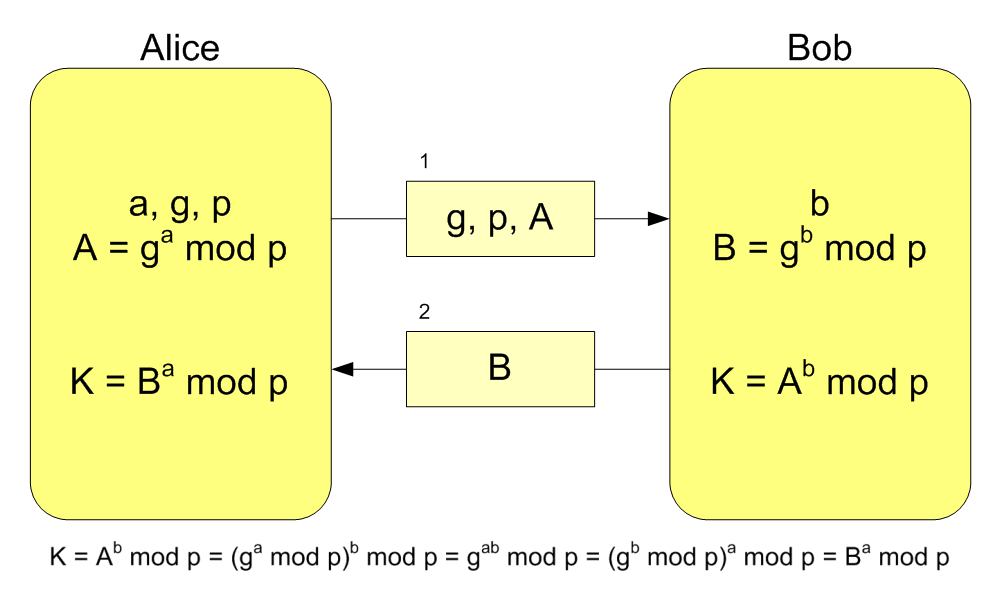
\includegraphics[width=0.6\textwidth]{./figure//D-H}
\caption{Scambio di chiavi Diffie-Hellman, schema di funzionamento.}
\label{FIG:DH}
\end{figure}

\subsubsection{TLS}
Il TLS (Transport Layer Security) � un protocollo crittografico, utilizzato su reti TCP/IP per cifrare delle comunicazioni tra due nodi. Esso viene ampiamente usato per proteggere e-mail, VoIP, web browsing ecc, quindi si occupa di cifrare le connessioni a livello di applicazione del modello ISO/OSI. Al suo interno sono stati implementati vari algoritmi per scambiare le chiavi in maniera sicura e per l'autenticazione come RSA e Diffie-Hellman, AES per la cifratura simmetrica, MD5 e SHA per il controllo dell'integrit� dei dati. Quando due sistemi vogliono comunicare tra loro attraverso TLS devono procedere in tre fasi:

\begin{itemize}
\item handshake e negoziazione tra le parti sugli algoritmi di cifratura da utilizzare (scambio della cipherlist o cipher suite);
\item scambio delle chiavi e autenticazione;
\item scambio di messaggi cifrati in maniera simmetrica e autenticati.
\end{itemize}

\subsubsection{HTTPS}
L'HTTPS (HyperText Transfer Protocol over Secure Socket Layer) � un protocollo per la comunicazione sicura, largamente utilizzato su internet. In pratica HTTPS consiste nella comunicazione tramite il protocollo HTTP all'interno di una connessione criptata da TLS. HTTPS garantisce l'autenticazione del sito web visitato, cifratura dei dati scambiati, protezione della privacy e integrit� dei dati.

\subsubsection{SHA}
SHA (Secure Hash Algorithm) indica una famiglia di cinque algoritmi crittografici, utilizzati per produrre una sorta di impronta digitale del messaggio, chiamato hash. Se indichiamo con $M$ un messaggio qualsiasi e con $\mathcal{H}$ la funzione di hash, allora $D=\mathcal{H}(M)$ sar� diversa per ogni $M'\ne M$. Generalmente algoritmi di questo tipo vengono utilizzati per verificare l'integrit� dei messaggi. Inviando l'hash di un messaggio, insieme al messaggio stesso, il destinatario pu� verificarne l'integrit� ricalcolando la funziona e confrontando il risultato con quello ricevuto dal mittente. Se il messaggio subisce modifiche prima di arrivare a destinazione, l'hash calcolato a destinazione sar� diverso da quello calcolato dalla sorgente.

%Ogni volta che viene scambiato un messaggio, viene anche inviato il suo hash, in modo che il destinatario possa verificare l'integrit� dello stesso ricalcolando la funzione e confrontando il risultato con quello ricevuto.


%diffusi

%\section{Protocolli crittografici}
%HTTPS, TLS, Diffie-Hellman, SHA-1
% ---- ELEMENTI UTILI E GIA' PRONTI! ----
%Secondo capitolo della tesi. Esempio di citazione doppia \cite{Munoz-Lipo,Vas}.

%Esempio di figura in \figurename\ \ref{FIG:LogoUniPD}.
%
%\begin{figure}[!htbp]
%\centering
%
\includegraphics[width=0.25\textwidth]{./figure//LogoUniPD}
%\caption{Esempio di figura.}
%\label{FIG:LogoUniPD}
%\end{figure}
%
%Esempio di tabella in \tablename\ \ref{TAB:Esempio}.
%
%\begin{table}[!htbp]
%\centering
%\renewcommand{\arraystretch}{1.3}
%\caption{Esempio di tabella.}
%\begin{tabular}{cc}
%\hline
%Nome & Valore \\
%\hline
%a & 1 \\
%b & 2 \\
%c & 3 \\
%d & 4 \\
%e & 5 \\
%f & 6 \\
%\hline
%\end{tabular}
%\label{TAB:Esempio}
%\end{table}

\clearemptydoublepage

\chapter{La rete Tor}
I messaggi trasmessi attraverso l'Onion Routing vengono crittografati a strati con metodi di crittografia simmetrica e inoltrati da dei router o relay, chiamati \emph{Onion Router} ($OR$), in cui � in esecuzione un processo a livello utente, che non necessita di privilegi particolari. Ogni client che vuole stabilire una connessione sicura con un host, deve prima costruire un tunnel attraverso la rete Tor utilizzando un particolare protocollo. Viene detta crittografia stratificata perch� man mano che il messaggio avanza nel tunnel, viene rimosso un livello crittografico, come spiegato nella Figura~\ref{FIG:strat}. Gli utenti che vogliono collegarsi alla rete devono utilizzare un software chiamato \emph{Onion Proxy} ($OP$) che stabilisce i circuiti all'interno della rete e gestisce le connessioni. Ogni router possiede una chiave a lungo termine, utilizzata per firmare i certificati TLS e le proprie caratteristiche che vengono divulgate pubblicamente (come bitrate, indirizzo, tipo ecc.). Inoltre possiede una chiave pubblica a breve termine o onion key usata dai client per crittografare le richieste che, come gi� detto, viene cambiata periodicamente. 

\subsubsection{Le cell}
La maggior parte dei dati scambiati tra due router o tra un router e un client avviene attraverso delle \emph{cell} di dimensione fissa. Esse sono dei pacchetti a livello di applicazione di dimensione fissa di 512 byte, formate da un header e da un payload. L'header contiene informazioni come il circID che serve per identificare il circuito al quale la cell � destinata o anche il CMD che indica cosa fare con il payload. Tutte le comunicazioni router-router e router-client avvengono attraverso delle connessioni TLS (pi� circuiti possono essere multiplati attraverso una connessione TLS). Esistono vari comandi che vengono inseriti nel campo CMD di una cell, ad esempio {\ttfamily CREATE} o {\ttfamily CREATED} usati per costruire un nuovo circuito, oppure {\ttfamily RELAY} che indica che la cell deve essere solo inoltrata al prossimo nodo ecc. Le cell di tipo  {\ttfamily RELAY} possiedono dei campi aggiuntivi all'interno dell'header come lo StreamID che identifica lo stream tra tutti quelli multiplati nel circuito oppure il Digest che serve per verificare l'integrit� dei dati.
\begin{figure}[!htbp]
\centering
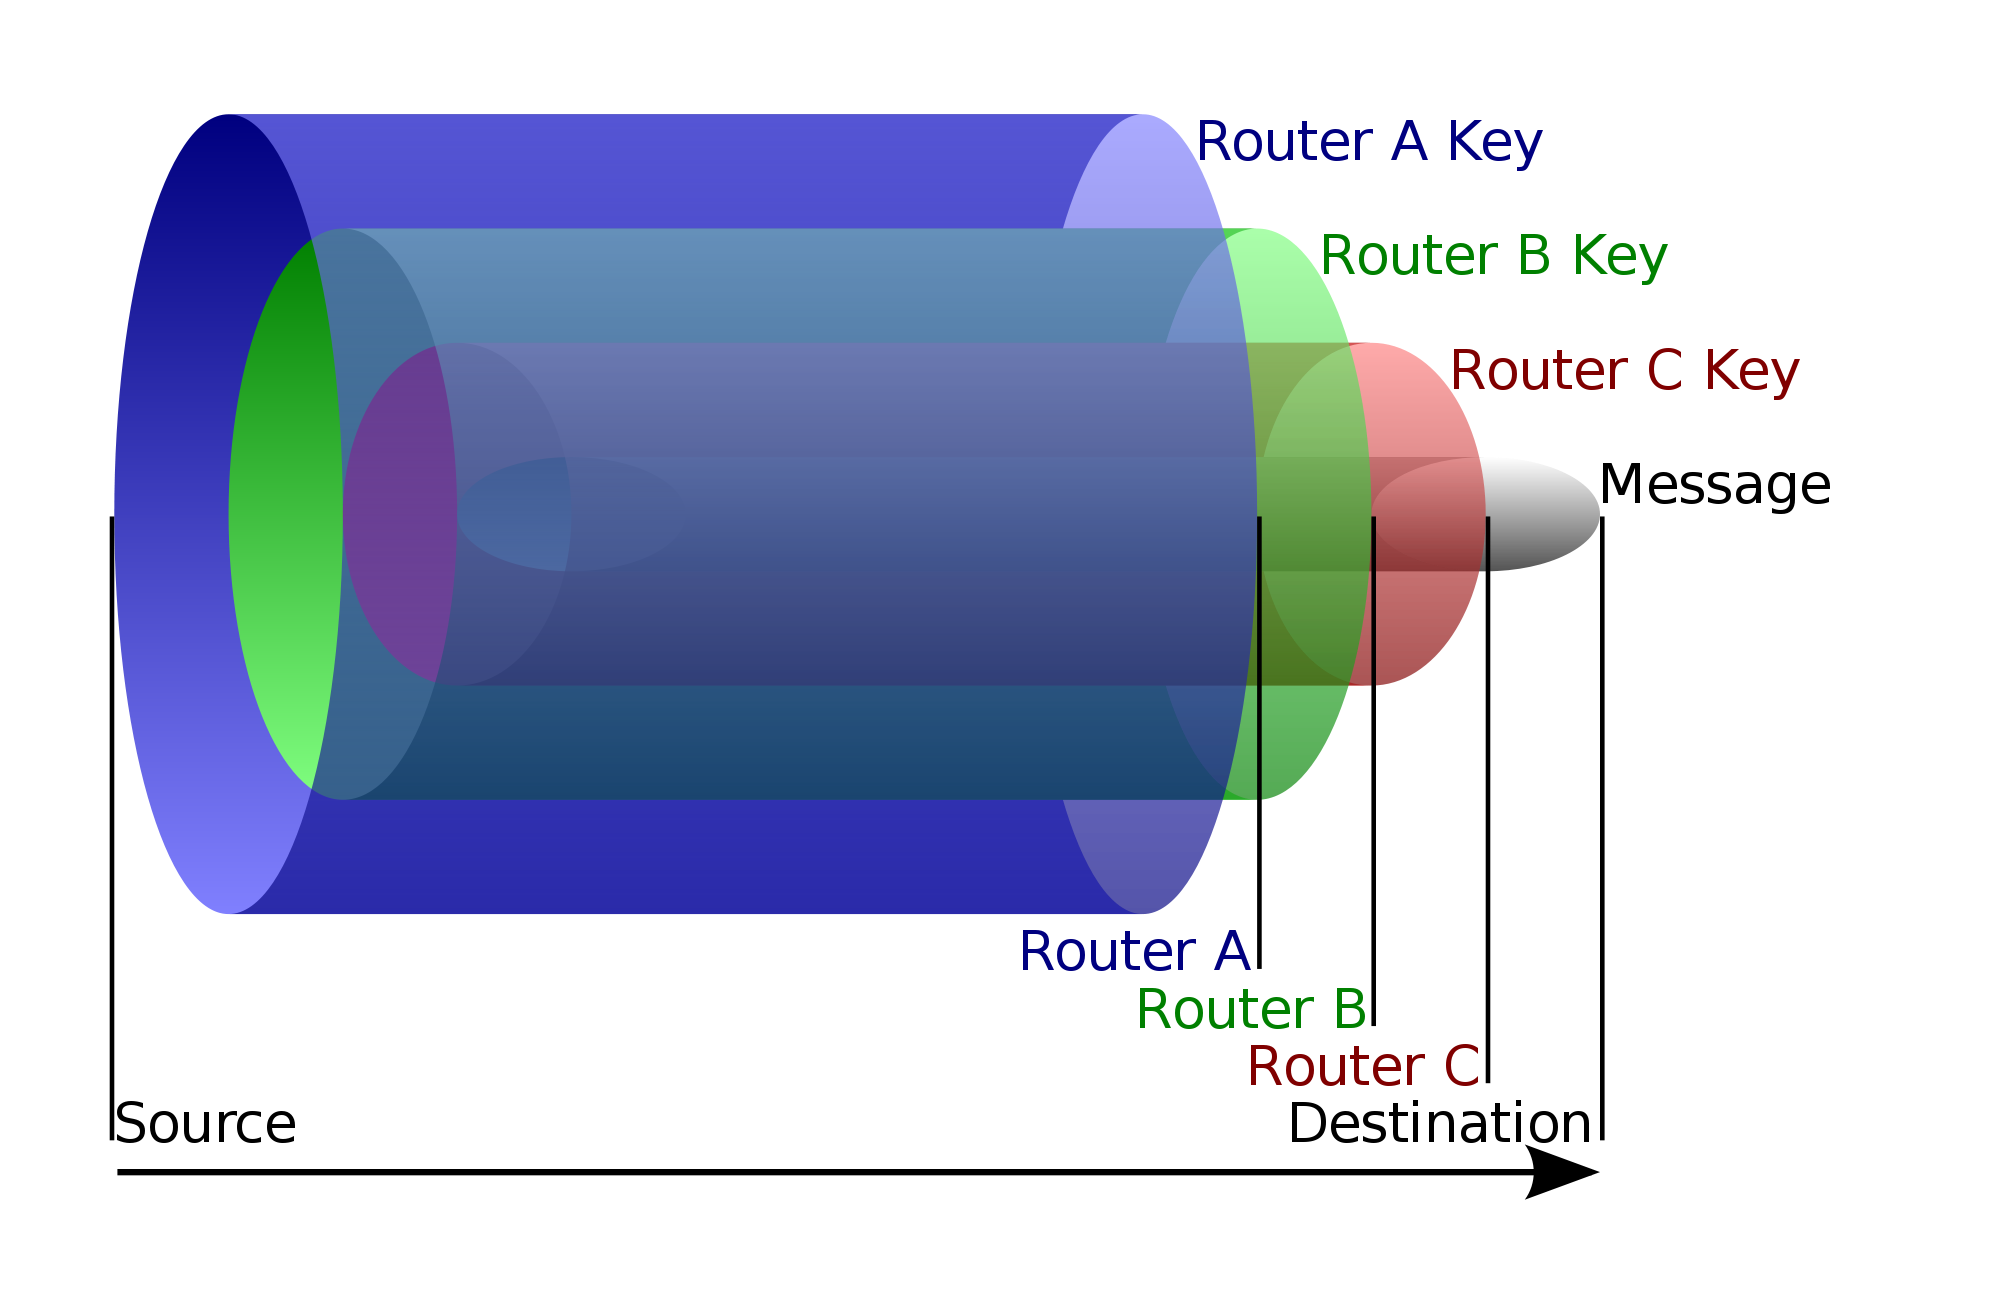
\includegraphics[width=0.5\textwidth]{./figure//strat}
\caption{Livelli di crittografia dell'onion routing.}
\label{FIG:strat}
\end{figure}

\section{Scelta dei nodi e costruzione del circuito}
\begin{figure}[!htbp]
\centering
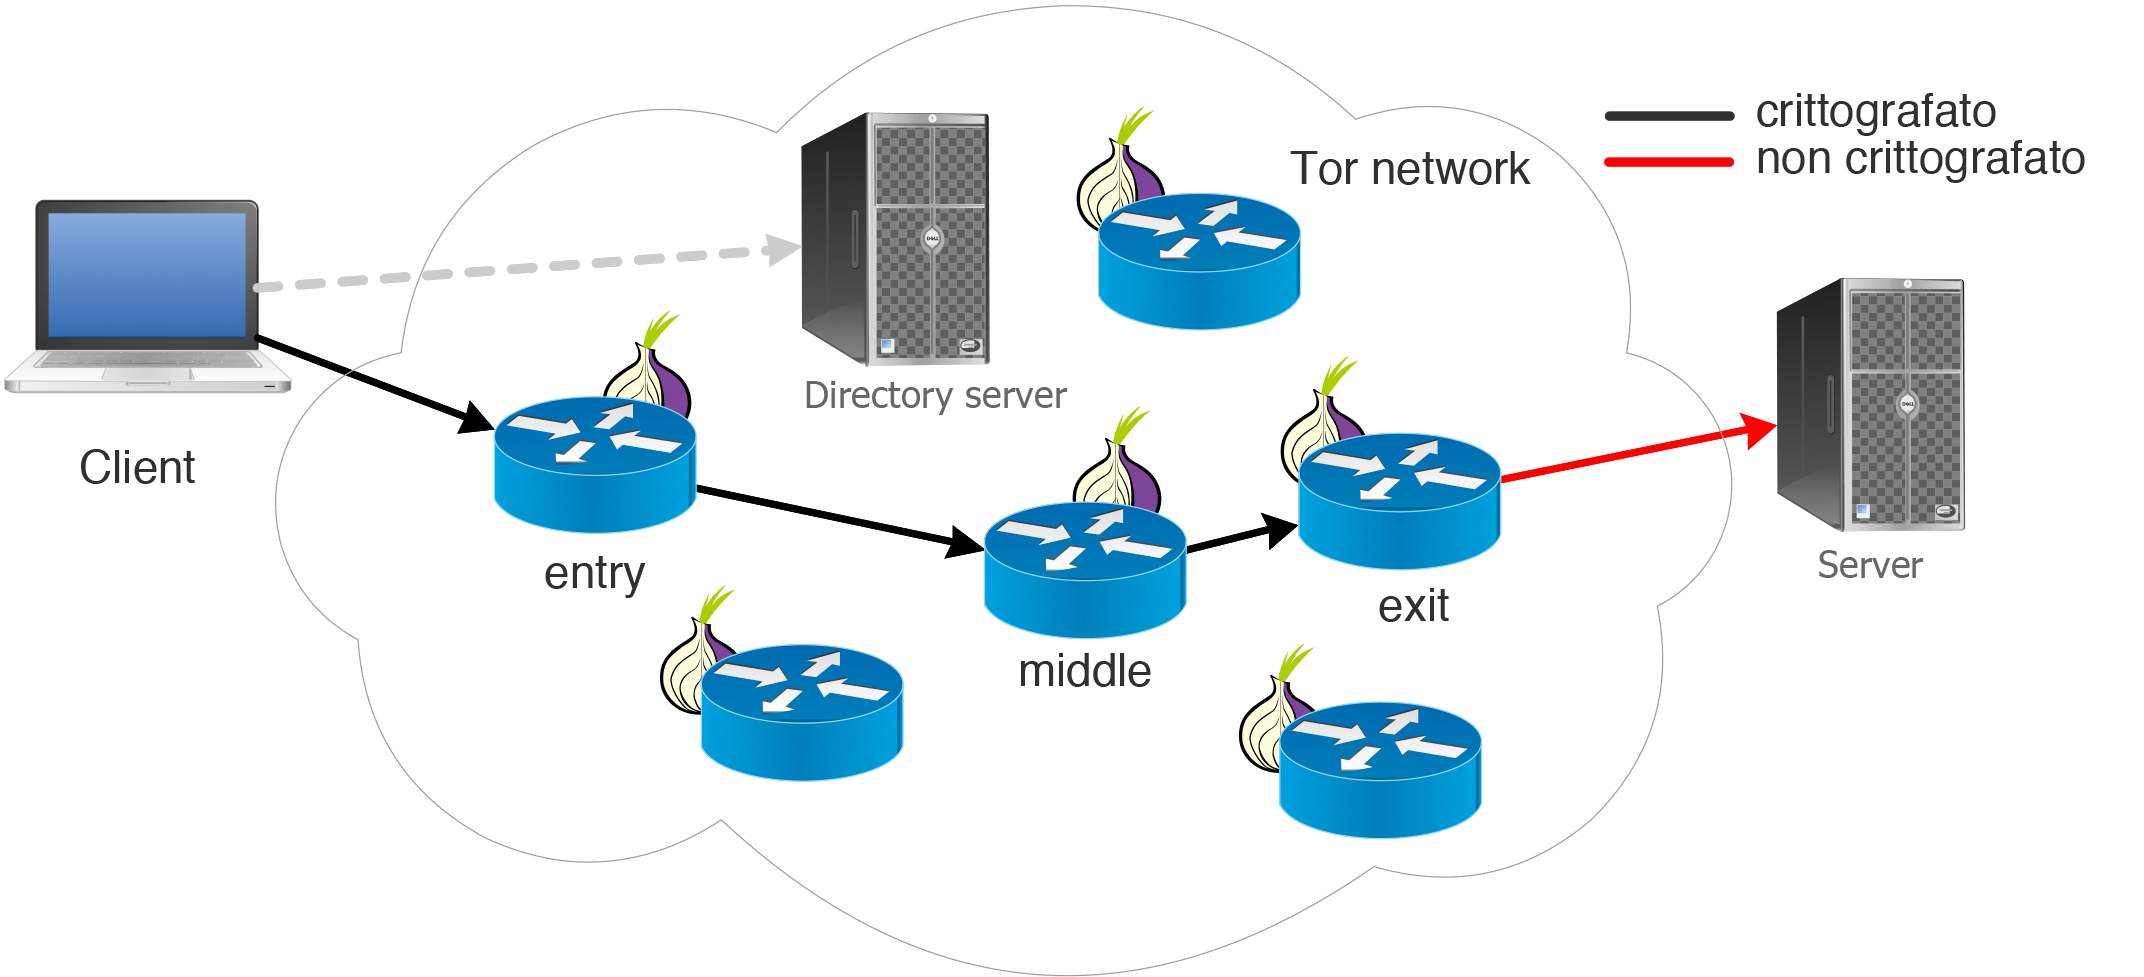
\includegraphics[width=0.7\textwidth]{./figure//tor}
\caption{Circuito Tor.}
\label{FIG:torcirc}
\end{figure}
L'Onion Proxy costruisce in maniera incrementale il circuito, scegliendo solitamente tre Onion Router tra tutti quelli disponibili. Per sapere quali relay sono disponibili in un dato momento, esistono dei \emph{directory server} che contengono una lista di tutti gli $OR$, comprensiva di indirizzo IP, bitrate offerto, chiave pubblica e altre informazioni. Come mostrato in Figura~\ref{FIG:torcirc} ogni circuito � costituito da un entry router, un middle e un exit. Per assicurare buone prestazioni essi vengono scelti tramite un algoritmo pesato di selezione che tiene conto del bitrate che ogni router annuncia.
I router possono essere suddivisi in quattro insiemi diversi: pure entry (o entry guard) ($G_{0}$), pure exit ($E_{0}$), sia entry che exit ($A$) e n� entry n� exit ($N_E$). 
Indichiamo con $i$ l' i-esimo router all'interno della rete con $i=1,2,...,N$ dove $N$ � il numero totale di onion router. Possiamo dare quindi le seguenti definizioni:
\begin{equation}
E_{0}=\{i: OR_{i} \, \text{� pure exit}\} \subset E \text{ con } E=\{i: OR_{i} \, \text{� exit}\} \subset \{\text{$1$, $2$,...,$N$}\} 
\end{equation}

\begin{equation}
 G_{0}=\{i: OR_{i} \, \text{� pure entry}\} \subset G \text{ con } G=\{i: OR_{i} \, \text{� entry}\} \subset \{\text{$1$, $2$,...,$N$}\}.
\end{equation}
 Da cui derivano le relazioni:
\begin{equation}
E=A \cup E_{0} \text{ e } G=A \cup G_{0}
\end{equation}
che indicano che gli entry router sono formati dall'unione dei pure entry e da quelli che possono operare sia da entry che da exit; la stessa cosa vale per gli exit.
Se $B_{i}$ rappresenta il bitrate dell' i-esimo router (uguale sia in ingresso che in uscita), il bitrate totale della rete sar� definita come:
\begin{equation}
B=\sum_{i=1}^N B_{i}
\end{equation}
mentre il bitrate totale di uscita, puramente di uscita, di ingresso e puramente di ingresso sono rispettivamente:
\[
B_{E}=\sum_{i\in E}B_{i} \text{ , } B_{E_0}=\sum_{i\in E_0}B_{i} \text{ , } B_{G}=\sum_{i\in G}B_{i} \text{ , } B_{G_0}=\sum_{i\in G_0}B_{i} \text{.}
\]
Per primo viene scelto il router di uscita e quindi bisogna definire un peso per il bitrate dei router $\in A$ (in quanto anche essi possono essere scelti come exit):

\begin{equation}
\label{eqn:wgpath}
W_G=
\begin{cases}
1-\frac{B}{3B_G},      	& \text{$altrimenti$,} \\
0, 									& \text{se $B_G < B/3$.}
\end{cases}
\end{equation}
Allora la probabilit� di scegliere l' i-esimo router, come router di uscita � definita come:

\begin{equation}
P_i=
\begin{cases}
\frac{B_i}{B_{E_{0}}+W_G B_A},      	& i \in E_0 \\
\frac{W_G B_i}{B_{E_{0}}+W_G B_A}, 	& i \in A.
\end{cases}
\end{equation}
Questo significa che, se ad esempio, il bitrate in ingresso � scarso ($B_G < B/3$), i router che possono operare sia da entry che da exit, non verranno considerati nel momento in cui verr� scelto il nodo di uscita. Per la scelta del router d'ingresso vale lo stesso ragionamento:

\begin{equation}
\label{eqn:wepath}
W_E=
\begin{cases}
1-\frac{B}{3B_E},      	& \text{$altrimenti$,} \\
0, 									& \text{se $B_E < B/3$}
\end{cases}
\end{equation}
e la probabilit� di scegliere un router come entry diventa:

\begin{equation}
P_i=
\begin{cases}
\frac{B_i}{B_{G_{0}}+W_E B_A},      	& i \in G_0 \\
\frac{W_E B_i}{B_{G_{0}}+W_E B_A}, 	& i \in A
\end{cases}
\end{equation}
con $B_{A}=\sum_{i\in A}B_{i}$.
Dopo aver scelto i router di uscita e di ingresso, si procede con la scelta del middle. Anche in questo caso vanno valutati i pesi prima di calcolare la probabilit� che venga scelto l'i-esimo router:

\begin{equation}
\bar{B_{i}} =
\begin{cases}
W_E B_i,      	& i \in E_0 \\
W_G B_i, 	& i \in G_0 \\
W_E W_G B_i, 	& i \in A \\
B_i,	& i \in N_E 
\end{cases}
 \text{ , } 
P_i=\frac{\bar{B_{i}}}{B_{E_{0}}W_{E}+B_{G_{0}}W_{G}+B_{A}W_{E}W_{G}+B_{N}}
\end{equation}
Una volta scelti i nodi che andranno a costituire il circuito, il client (Alice nella Figura~\ref{FIG:circbuild}) invia una {\ttfamily CREATE} cell al router d'ingresso, contenente la prima met� dell'handshake ($g^x$) di Diffie-Hellman, crittografata con l'onion key. L'$OR_{1}$ deve quindi decifrare la richiesta e rispondere con una {\ttfamily CREATED} cell contenente ($g^y$) insieme all'hash della chiave negoziata $K=g^{(xy)}$. Da questo momento in poi Alice e l'entry router potranno comunicare utilizzando un algoritmo di crittografia simmetrica (tipicamente AES) con la chiave appena concordata. Per estendere il circuito, il client deve inviare una {\ttfamily RELAY\textunderscore EXTEND} cell al router d'ingresso, comprensiva dell'indirizzo del prossimo relay e della prima met� della dell'handshake di Diffie-Hellman ($g^{x_{2}}$). L'entry copia il mezzo handshake in una {\ttfamily CREATE} cell e la inoltra al middle router. Quando l'$OR_{2}$ risponde con la {\ttfamily CREATED} cell, l'$OR_{1}$ copia il payload all'interno di una  {\ttfamily RELAY\textunderscore EXTENDED} cell e la invia ad Alice. Adesso anche Alice e il middle router condividono una chiave $K_{2}=g^{(x_{2}y_{2})}$ da utilizzare per comunicare tra di loro. Per estendere ulteriormente il circuito, viene ripetuta la procedura appena descritta, comunicando il comando di estensione all'ultimo router. Normalmente, quando due router o un router e il client devono comunicare tra di loro, utilizzano le {\ttfamily RELAY} cell. Quando il client fa una richiesta, ad esempio ad un server web che si trova al di fuori della rete Tor, essa viene incapsulata in una {\ttfamily RELAY} cell, crittografata sequenzialmente con le chiavi di sessione e inviata all'entry. La cell deve percorrere il circuito dal primo all'ultimo router, ognuno dei quali si occupa di rimuovere un livello di crittografia. L'ultimo router, oltre a rimuovere l'ultimo livello, inoltra la richiesta al server e riceve la risposta. Una volta ricevuta la risposta, anch'essa viene incapsulata in una cell, crittografata con la chiave di sessione e rispedita al nodo precedente, proseguendo allo stesso modo attraverso gli altri nodi. Il nodo di uscita quindi esegue le operazioni per conto del client, aprendo una connessione in genere non crittografata con gli host esterni alla rete Tor. Grazie al meccanismo appena descritto, il client pu� rimanere in totale anonimato, poich� ogni router conosce solo i due nodi con i quali sta comunicando, ma non conosce gli altri componenti del circuito.
\begin{figure}[!htbp]
\centering
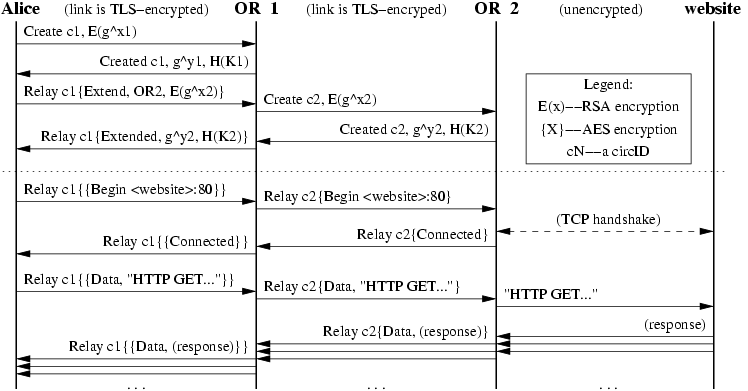
\includegraphics[width=0.9\textwidth]{./figure//circuit-building}
\caption{Procedura per la costruzione di un circuito e richiesta ad un server web.}
\label{FIG:circbuild}
\end{figure}

\newpage
\section{Servizi Nascosti}
Oltre a garantire l'anonimato ai client, Tor � in grado di fare la stessa cosa lato server. Questo significa che � possibile fornire un servizio (come ad esempio un sito web), facendo in modo che la localizzazione del server rimanga sconosciuta. Per accedere ad un servizio nascosto, un client deve obbligatoriamente utilizzare Tor, e deve riferirsi ad esso attraverso un pseudo dominio di primo livello ".onion". Quando un nuovo servizio viene attivato, esso deve comunicare la propria esistenza alla rete per poter essere raggiungibile dai client. Per prima cosa deve stabilire dei \emph{punti di introduzione}, cio� scegliere in maniera casuale dei router e costruire dei circuiti che terminano in questi ultimi, comunicandogli di rimanere in attesa di richieste. Successivamente viene inviato ad un database, un \emph{descrittore} (firmato con la chiave privata), contenente la chiave pubblica e un elenco dei punti di introduzione.\\ Quando un client (Alice) tenta di contattare un servizio nascosto (Bob), vengono eseguite le seguenti operazioni:
\begin{enumerate}
\item Alice esegue una chiamata all'indirizzo xyz.onion, per ottenere il descrittore del servizio e conoscere cos� i suoi punti di introduzione (xyz � una sequenza di 16 caratteri derivante dalla chiave pubblica del servizio stesso); 
\item Alice sceglie un $OR$ come \emph{punto di rendezvous}  da utilizzare per connettersi al servizio;
\item  Alice apre un circuito anonimo con uno dei punti di introduzione per comunicare al servizio il punto di rendezvous scelto e la prima met� dell'handshake di DH;
\item se Bob accetta la richiesta, si connette al punto di rendezvous e comunica ad Alice la seconda met� dell'handshake di DH e un hash della chiave concordata;
 \item adesso il punto di rendezvous collega il circuito di Alice con quello di Bob, che potranno comunicare in maniera del tutto anonima.
\end{enumerate}



%\begin{enumerate}
%\item eseguire una chi
%\end{enumerate}

%\lipsum[1-2]
%%%%% authority tor


% ---------------------  ESEMPI UTILI PRONTI ALL'USO  ----------------------------
%TERZO capitolo della tesi. Esempio di citazione doppia \cite{Munoz-Lipo,Vas}.
%
%Esempio di figura in \figurename\ \ref{FIG:LogoUniPD}.
%
%\begin{figure}[!htbp]
%\centering
%
\includegraphics[width=0.25\textwidth]{./figure//LogoUniPD}
%\caption{Esempio di figura.}
%\label{FIG:LogoUniPD}
%\end{figure}
%
%Esempio di tabella in \tablename\ \ref{TAB:Esempio}.
%
%\begin{table}[!htbp]
%\centering
%\renewcommand{\arraystretch}{1.3}
%\caption{Esempio di tabella.}
%\begin{tabular}{cc}
%\hline
%Nome & Valore \\
%\hline
%a & 1 \\
%b & 2 \\
%c & 3 \\
%d & 4 \\
%e & 5 \\
%f & 6 \\
%\hline
%\end{tabular}
%\label{TAB:Esempio}
%\end{table}

\clearemptydoublepage

\chapter{Blanket blocking}
Il \emph{blanket blocking} � un attacco che permette di bloccare l'accesso all'intera rete Tor e viene solitamente attuato da enti governativi, ISP o amministratori di rete. Esso non intende colpire un router o un client specifico, ma attraverso l'utilizzo di firewall o filtri impedisce l'accesso a chiunque si voglia collegare alla rete Tor.
%Esistono vari metodi che impediscono l'accesso alla rete:
%\begin{itemize}
%\item bloccando le connessioni verso le directory authorities;
%\item bloccando le connessioni verso i router distribuiti dalle directory authorities;
%\item filtrando i pacchetti che nell'header HTTP contengono dei riferimenti a Tor;
%\item bloccando l'accesso al sito ufficiale di Tor, per diminuire il numero di download del software;
%\item \textcolor{green}{tecniche DPI}
%\end{itemize}
Esistono principalmente due metodi per impedirne l'accesso:
\begin{itemize}
\item blocco delle connessioni verso le infrastrutture di Tor (\emph{address-blocking});
\item utilizzo di tecniche DPI (\emph{content-based blocking}).
\end{itemize}
Per attuare il primo metodo, un ISP (ad esempio) pu� semplicemente inserire in una blacklist tutte le coppie IP:porta delle directory authorities, gli IP distribuiti da esse o l'IP del server che ospita il sito \url{https://www.torproject.org/} (per impedire che il software si diffonda). Ogni qualvolta si tenter� di stabilire una connessione verso uno di questi indirizzi IP, verr� impedito ai pacchetti di raggiungere il server, oppure di ricevere le risposte. Con le tecniche DPI (Deep Packet Inspection) i pacchetti vengono analizzati da software specifici in grado di individuare il contenuto del pacchetto o l'applicazione che l'ha generato (in questo caso Tor) e scartarli per impedire che arrivino a destinazione. Nel caso di Tor, solitamente, viene individuato il protocollo nel momento in cui il client invia la cipher list al primo router, contenuta nel TLS hello\footnote{Il TLS hello � la prima fase dell'handshake TLS, in cui il client comunica al server (o al router in questo caso) gli algoritmi crittografici supportati, la versione TLS ecc.}. Infatti la cipher list sembra essere unica ed utilizzata solamente da Tor.

\section{Bridge}
Il metodo pi� semplice per difendersi da questo tipo di attacco consiste nell'utilizzare i bridge. Essi sono dei router Tor, che non vengono inseriti nelle liste delle directory authorities. Dato che i loro indirizzi IP non sono pubblici, non vengono censurati e quindi � possibile utilizzarli come first-hop per collegarsi alla rete Tor. Per ovvi motivi vengono messi a disposizione dei metodi che permettono di ottenere solamente pochi bridge alla volta. Inviando un' email a \mail{bridges@torproject.org} da un account Riseup, Gmail o Yahoo si ottiene una risposta con tre indirizzi IP di tre bridge diversi. Oppure vengono distribuiti attraverso server HTTPS come \url{https://bridges.torproject.org/}, social networks o canali privati. 

Un metodo molto pi� sofisticato \cite{torbridge} per raccogliere gli indirizzi IP dei bridge, � quello di utilizzare un middle router controllato che raccolga informazioni sugli altri router della rete: inserendo all'interno della rete un router con un bitrate elevato si avr� un alta probabilit� che esso venga scelto come middle nelle costruzioni dei path. Cos� facendo il router controllato pu� confrontare gli indirizzi IP dei nodi di ingresso con quelli delle directory authorities. Se l'indirizzo confrontato non � presente tra quelli pubblici allora il router d'ingresso � un bridge e quindi pu� essere comunicato attraverso un'email ad un indirizzo prestabilito. Quando gli onion router notano che il bitrate e l'uptime del router controllato stanno al di sopra di un valore medio, esso viene etichettato come entry router dai directory server. Per evitare che il nodo inserito all'interno della rete diventi un entry bisogna regolare il bitrate e l'uptime dinamicamente, mentre per evitare che diventi un exit � necessario indicarlo in fase di configurazione.
% FIGURA
\begin{figure}[!htbp]
\centering
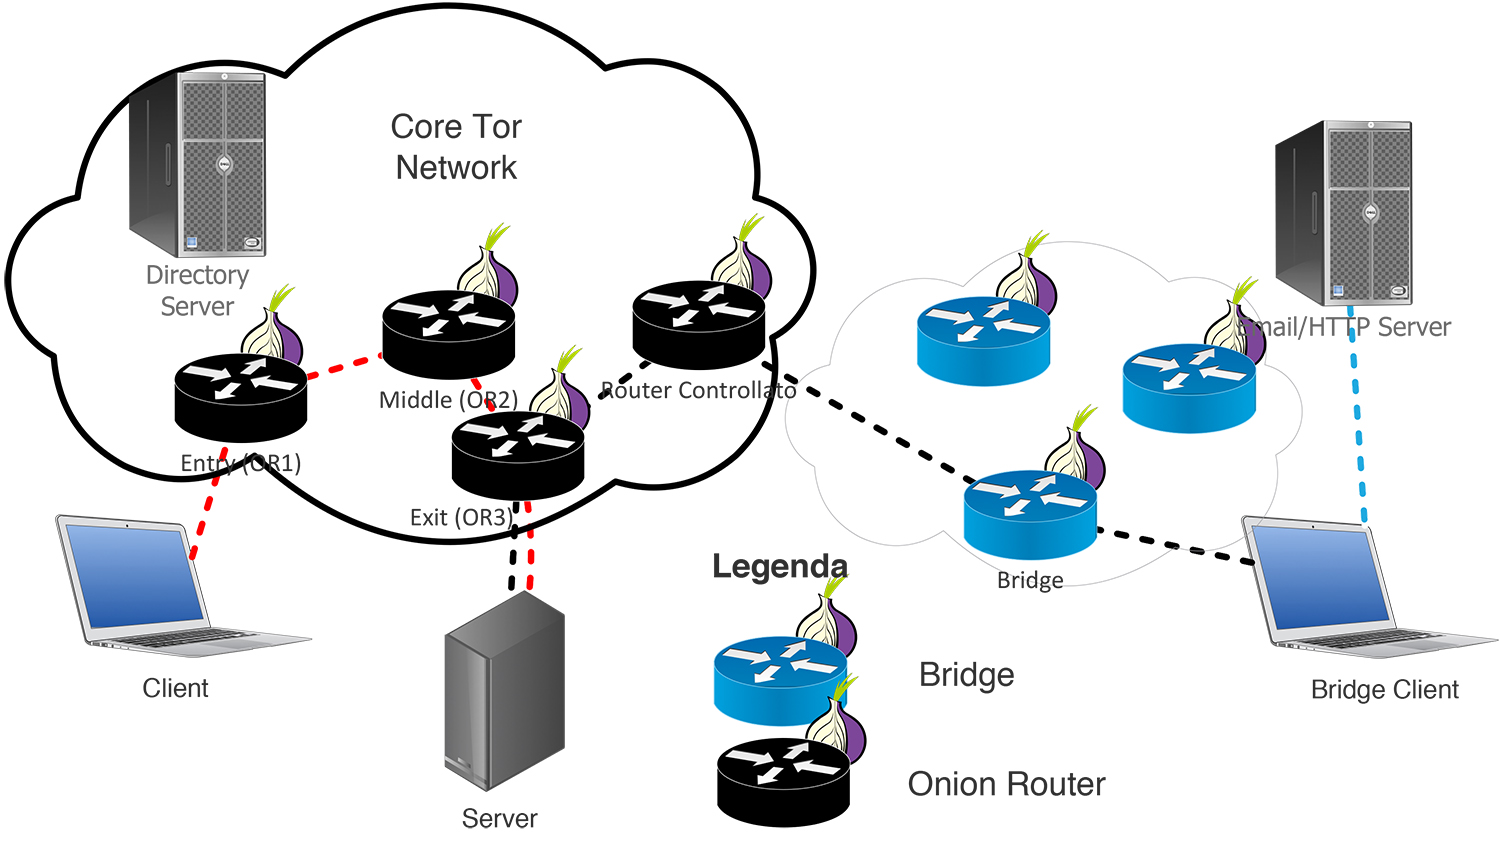
\includegraphics[width=0.6\textwidth]{./figure//middleroutercut2}
\caption{Scenario di rete con router controllato.}
\label{FIG:TorBridge}
\end{figure}
\\Analizziamo allora la \textbf{probabilit� di cattura}, ovvero la probabilit� che un circuito che sceglie come first-hop un bridge, attraversi il router controllato. Ipotizziamo di inserire $k$ middle router nella rete e che il numero totale di OR fino a quel momento fosse $N$, allora i rispettivi bitrate li indicheremo con $\{B\ped{1},B\ped{2}, ... , B_{k}, B_{k+1}, ... , B_{k+N}\}$. Tutti i router inseriti avranno lo stesso bitrate, $B_1 = B_2 = ... = B_k = b$. Definiamo $B$ come la somma dei bitrate di tutti gli OR originariamente presenti nella rete: $B = \sum_{i=k+1}^{k+N} B_i$. Quindi dopo l'inserimento, il bitrate totale sar� $B+k \cdot b$. Da \eqref{eqn:wepath} e \eqref{eqn:wgpath} possiamo scrivere:

\begin{equation}
W_E=
\begin{cases}
1-\frac{B+k \cdot b}{3 \cdot (B_{E0}+B_A)},      	& \text{se $W_E>0$,} \\
0, 									& \text{se $W_E\le0$.}
\end{cases}
\end{equation}

\begin{equation}
W_G=
\begin{cases}
1-\frac{B+k \cdot b}{3 \cdot (B_{G0}+B_A)},      	& \text{se $W_G>0$,} \\
0, 									& \text{se $W_G\le0$.}
\end{cases}
\end{equation}
Diamo allora la definizione di probabilit� di cattura:

\begin{teorema}[Probabilit� di cattura]
\begin{equation}
\label{eqn:probcatch}
P(k,b) = \frac{k\cdot b}{B_{E0} \cdot W_E + B_A \cdot W_E \cdot W_G + B_{G0} \cdot W_G + (B_N+ k \cdot B)}
\end{equation}
\end{teorema}
Da qui deriva immediatamente che pi� � grande il bitrate portato all'interno della rete, pi� probabilit� si ha di essere scelti nei circuiti Tor, come enunciato dal seguente teorema.

\begin{teorema}
La probabilit� di cattura � determinata dall'ammontare del bitrate aggiunto dagli $OR$ controllati. Sia $M = k \cdot b, M' = k' \cdot b' \ con \ M \ge M'$,
\begin{equation}
\label{eqn:ammband}
P(M) \ge P(M').
\end{equation}
L'uguaglianza si ha con $M'=M$.
\end{teorema}

\begin{teorema}
Dopo la creazione di q circuiti, la probabilit� che almeno uno dei bridge si sia collegato ad uno dei router controllati �:
\begin{equation}
\label{eqn:ammband}
P(k,b,q) = 1- (1-P(k,b))^{q}, \ q=1,2,3,...
\end{equation}
\end{teorema}
In conclusione, la probabilit� di cattura aumenta con l'aumentare del bitrate totale dei router controllati e con il numero di circuiti che vengono creati.
Come � stato evidenziato sperimentalmente \cite{torbridge}, in pochi giorni con un solo router si � in grado di raccogliere un numero considerevole di bridge.

\section{Pluggable transports}
Il semplice uso dei bridge si oppone solo alla censura a livello IP e non va a contrastare, laddove vengono utilizzate, le tecniche DPI. Come abbiamo detto il Deep Packet Inspection va ad analizzare il contenuto dei pacchetti, ma � possibile camuffarli con dei tool detti \emph{pluggable transports}  in modo da aggirare i blocchi di tipo content-based.
Possono essere scelte due strategie per camuffare i pacchetti:
\begin{itemize}
\item far sembrare il flusso di pacchetti qualcosa che non viene bloccato;
\item far sembrare il flusso di pacchetti qualcosa di autorizzato.
\end{itemize}
Dei tool che realizzano la prima strategia sono: obfs2, obfs3, ScrambleSuit e obfs4 che cercano di camuffare i pacchetti facendo sembrare lo stream di byte un insieme uniforme di bit casuali, inoltre fanno in modo che non rimanga nessuna parte della comunicazione in chiaro, neanche nella fase di handshake TLS e nello scambio delle chiavi. Anche se � possibile decifrare lo stream, questo richiederebbe ulteriori risorse che non vengono impiegate nella maggior parte dei casi. Questo metodo richiede che il tool sia eseguito sia sul client che sul bridge a cui ci si vuole collegare.
Nel secondo caso vengono usate tecniche steganografiche, che "trasformano" lo stream di dati di Tor, in uno stream simile a quello di altre applicazioni com ad esempio Skype.  

\section{Great Firewall of China (GFC)}
\emph{Great Firewall of China} � un termine utilizzato per far riferimento al \emph{Golden Shield Project}, un progetto per il controllo e la censura di Internet sviluppato dal governo cinese. Esso merita un approfondimento a parte per quanto riguarda l'aspetto tecnico data la sua efficacia nel realizzare il blanket blocking. Ogni volta che un client all'interno del territorio cinese tenta di collegarsi ad un $OR$, un blocco DPI identifica il protocollo Tor durante lo scambio della cipher suite TLS e lo comunica a dei server. Questi server provano a collegarsi all'$OR$ con lo stesso protocollo e, se ci riescono, lo inseriscono in una blacklist. Questo vale anche quando qualcuno ci si collega ad un bridge, rendendoli quindi inutilizzabili. I directory authorities vengono bloccati a livello IP, infatti non rispondono n� a pacchetti TCP n� ICMP. Attualmente il GFC sembra lasciar passare il TCP SYN, ma eliminare il SYN/ACK inviato dal router al client e la stessa cosa sembra succedere quando si prova a collegarsi ad un bridge bloccato. Comunque il blocco di router e bridge sembra riferirsi alle tuple IP:porta, dato che essi rispondono al ping verso altre porte. Probabilmente questa scelta � stata fatta per minimizzare gli effetti collaterali dovuti alla censura.

\subsection{Contromisure}
I risultati sperimentali \cite{gfc} mostrano che una tupla IP:Porta rimane bloccata fintanto che � raggiungibile. Questo significa che periodicamente i server del GFC provano a stabilire delle connessioni con i router/bridge che avevano precedentemente inserito nella blacklist. Se vedono che non sono pi� raggiungibili rimuovono il blocco. Questo meccanismo pu� essere sfruttato per aggirare il firewall. Si pu� pensare di inserire un router all'interno della rete Tor posizionato al di fuori del territorio cinese e configurarlo in modo che accetti solo connessioni da degli indirizzi IP prestabiliti. Cos� facendo anche se i blocchi DPI rilevassero l'uso del protocollo Tor verso il router, i server del GFC non potrebbero provare a collegarsi dato che le loro richieste verrebbero scartate e quindi non bloccherebbero il router.

Il progetto Tor ha anche sviluppato un tool chiamato \emph{meek} \cite{meek, domainfronting} in grado di codificare uno stream di dati come una sequenza HTTPS di richieste e risposte che vengono inoltrate da un web server; questa tecnica � detta \emph{domain fronting}.
% FIGURA
\begin{figure}[!htbp]
\centering
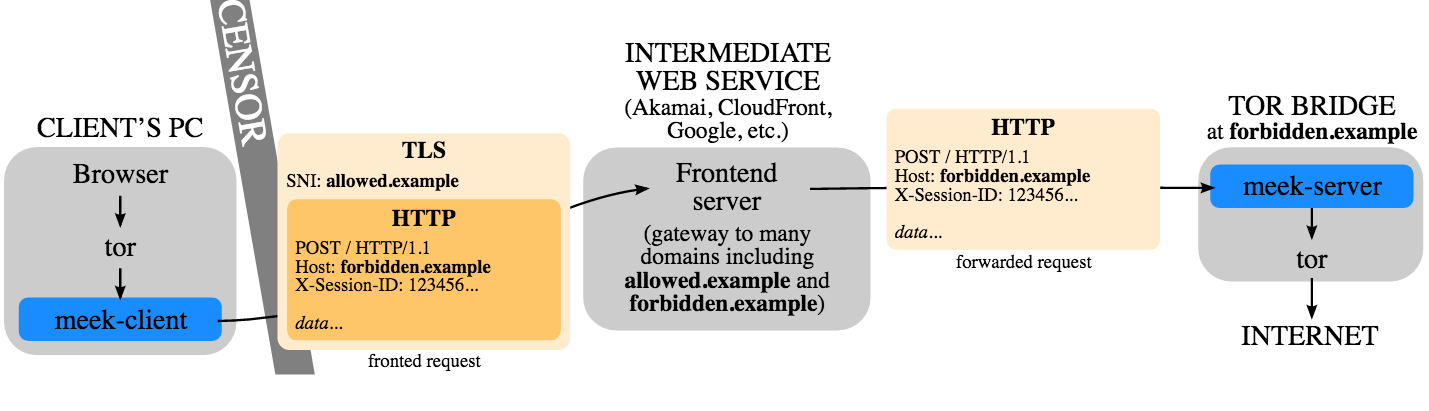
\includegraphics[width=0.9\textwidth]{./figure//meek-diagram}
\caption{Schema di funzionamento del tool meek.}
\label{FIG:meek}
\end{figure}
Il server quindi ha la funzione di intermediario e permette ad un client di collegarsi ad un Tor bridge, facendo sembrare che le richieste vadano verso un IP autorizzato. Meek si compone di due parti: meek-client e meek-server. La parte client � un processo separato rispetto al browser Tor che riceve i dati da trasmettere da esso, li "impacchetta" dentro ad una richiesta POST e li invia al bridge attraverso il web server. Il dominio autorizzato viene messo "all'esterno" della richiesta: nella query DNS e nell'estensione SNI TLS \footnote{L'estensione SNI (Server Name Indication) � un'estensione del protocollo TLS con cui un client indica a quale hostname sta cercando di connettersi all'inizio della fase di handshake.}, mentre il dominio vietato "all'interno": nell' host header della richiesta HTTP. Sul bridge � in esecuzione la parte server di meek, che decodifica le richieste HTTP in ingresso e le invia nella rete Tor. Dopo aver ricevuto una richiesta, meek-server controlla se il bridge ha dei dati da inviare come risposta al client, e li invia nella risposta HTTP; quando meek-client riceve la risposta, ne passa il corpo al processo Tor. Il motivo per cui questi web server non vengono bloccati � che fanno parte di qualche CDN, chi censura quindi, incapace di distinguere tra traffico fronted e non fronted, � costretto a scegliere: permettere il passaggio di traffico che aggira i firewall o bloccare completamente interi domini, con pesanti effetti collaterali. 


% ----------------------  ESEMPI UTILI PRONTI ALL'USO  ----------------------
%QUARTO capitolo della tesi. Esempio di citazione doppia \cite{Munoz-Lipo,Vas}.
%
%Esempio di figura in \figurename\ \ref{FIG:LogoUniPD}.
%
%\begin{figure}[!htbp]
%\centering
%
\includegraphics[width=0.25\textwidth]{./figure//LogoUniPD}
%\caption{Esempio di figura.}
%\label{FIG:LogoUniPD}
%\end{figure}
%
%Esempio di tabella in \tablename\ \ref{TAB:Esempio}.
%
%\begin{table}[!htbp]
%\centering
%\renewcommand{\arraystretch}{1.3}
%\caption{Esempio di tabella.}
%\begin{tabular}{cc}
%\hline
%Nome & Valore \\
%\hline
%a & 1 \\
%b & 2 \\
%c & 3 \\
%d & 4 \\
%e & 5 \\
%f & 6 \\
%\hline
%\end{tabular}
%\label{TAB:Esempio}
%\end{table}

\clearemptydoublepage

\chapter{Targeted Attack}
I \emph{targeted attack}, al contrario del blanket blocking, non riescono a bloccare completamente l'accesso alla rete, ma possono comunque causare un calo di prestazioni, di affidabilit� e di sicurezza rendendo inutilizzabili i nodi pi� importanti della rete. Nelle sezioni successive verranno descritti vari tipi di attacchi, le loro conseguenze e, per ognuno, discusse delle specifiche contromisure.
\section{CellFlood Attack}
Il CellFlood \cite{cellflood} � un attacco DoS selettivo, che permette di sovraccaricare la CPU di un Onion Router in maniera molto rapida, richiedendo un basso costo in termini di risorse alla macchina dell'aggressore. Esso sfrutta una vulnerabilit� nel protocollo di Tor, che si manifesta nella fase di costruzione di un circuito. Gli autori dello studio affermano che questo attacco � in grado di \emph{dimezzare} la capacit� di processing del 62\% degli $OR$ pi� usati di tutta la rete; inoltre richiede solamente un bitrate compreso tra 2.6 e 9.76 Mb/s per router che � molto inferiore rispetto a quello richiesto da un classico attacco DoS.

Ricordiamo che, ogni volta che si aggiunge un $OR$ al circuito, il client invia una {\ttfamily RELAY\textunderscore EXTEND} cell all'ultimo router $OR_{i}$ contenente un'\emph{onionskin} indicata con $E(g^x)$, dove $E(\cdot)$ indica la crittografia con l'\emph{onion key} pubblica RSA a 1024-bit, precedentemente scaricata da un'authority Tor. Una volta ricevuta la cell, l'$OR_{i}$ estrae l'onionskin e la invia al router da aggiungere $OR_{i+1}$ nel payload di una {\ttfamily CREATE} cell. Una volta che l'$OR_{i+1}$ decifra l'onionskin, risponde all'$OR_{i}$ con una {\ttfamily CREATED} cell, che viene incapsulata e inoltrata al client in una  {\ttfamily RELAY\textunderscore EXTENDED} cell.

L'operazione di processing dell'onionskin, � molto pi� costosa in termini di risorse rispetto alla sua creazione da parte del client, infatti decifrare con una chiave privata a 1024-bit occupa circa 20 volte il tempo necessario a cifrare con la corrispondente chiave pubblica a 1024-bit. Per questo motivo si spende $\sim 4$ volte pi� tempo a processare una {\ttfamily CREATE} cell piuttosto che generarla.
Tutto questo pu� essere sfruttato da un client aggressore che pu� consumare tutte le risorse di un Onion Router sommergendolo di {\ttfamily CREATE} cell. Inoltre non � necessario che ogni volta il client calcoli le nuove onionskin, ma pu� utilizzare sempre la stessa dato che l'$OR$ sar� costretto comunque a processarle una ad una. Nel software Tor in esecuzione negli $OR$, il main thread si occupa del pi� importante compito di inoltrare le {\ttfamily RELAY\textunderscore DATA} cell, mentre uno o pi� thread, chiamati CPU Workers, si occupano di processare le onionskin. Questa scelta di progettazione permette all'Onion Router di continuare ad inoltrare le cell anche se nello stesso momento viene inondato di {\ttfamily CREATE} cell. Se per� il rate di arrivo diventa pi� alto di quanto la CPU � in grado di processare, allora esse vengono scartate e viene risposto con una {\ttfamily DESTROY} cell. Questo causa un interruzione del servizio per tutti i client legittimi che vogliono stabilire una connessione con l'$OR$. Quindi se il CellFlood venisse utilizzato in maniera strategica, contro un insieme di router importanti, la parte rimanente della rete verrebbe sovraccaricata, oppure i tunnel costruiti da quel momento in poi potrebbero passare per degli $OR$ controllati, con una conseguente diminuzione di affidabilit�, sicurezza e QoS.
Un aggressore interessato ad attaccare un router, oppure un insieme di router, avrebbe a disposizione una tecnica pi� potente e meno costosa rispetto ad un classico attacco DoS a livello di rete.
%questo la rende circa 20 volte pi� lenta di un'operazione che utilizza la una chiave 
%\newpage

\begin{figure}[!htbp]
\centering
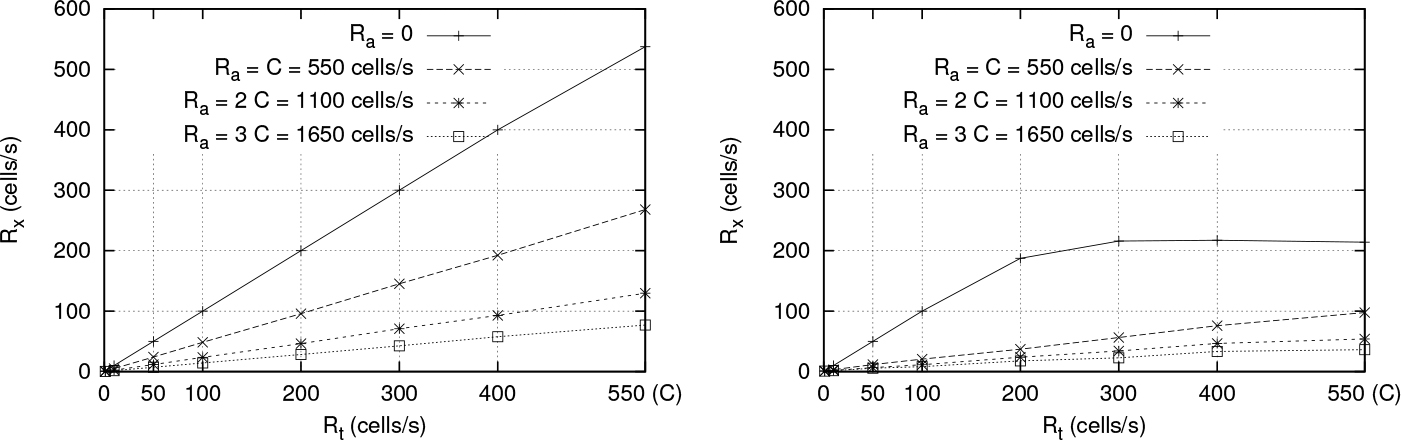
\includegraphics[width=0.95\textwidth]{./figure//cellflood}
\caption[Effetto di un CellFlood su un Onion Router.]{Effetto di un CellFlood su un $OR$, a sinistra senza traffico dati, mentre a destra con traffico dati. $R_{t}$ indica il rate di cell benigne, $R_{a}$ dell'aggressore, $R_{x}$ quelle effettivamente processate.}
\label{FIG:ClientPuzzles}
\end{figure}

\subsection{Difesa attraverso l'uso dei Client Puzzles}
Come contromisura al CellFlood Attack, sempre gli autori di \cite{cellflood} propongono una soluzione basata sui \emph{client puzzles}. Per fare in modo che il carico sulla CPU non vada fuori controllo, � stato pensato di far processare le onionskin al router, solo dopo che il client ha risolto un problema (tipicamente crittografico) che richiede una certa quantit� di risorse computazionali. Costringere il client a risolvere ogni volta un problema di questo tipo, riduce in maniera importante l'efficacia dell'attacco. I client puzzles sono un'ottima soluzione per difendere gli $OR$ per vari motivi:
\begin{itemize}
\item ogni router pu� difendersi indipendentemente, senza cooperare con gli altri $OR$, con il rischio che un altro qualsiasi possa essere controllato; 
\item l'efficacia dei client puzzles non dipende da come l'attacco � stato organizzato: pu� arrivare direttamente da un altro router o da un client, oppure indirettamente attraverso un altro router, incapsulando le onionskin in una {\ttfamily RELAY\textunderscore EXTEND} cell invece che in una {\ttfamily CREATE} cell;
\item le connessioni attive sul router sotto attacco non vengono chiuse;
\item possiedono un livello di difesa modulare, nel senso che la loro complessit� pu� essere modificata in base all'entit� dell'attacco, rimanendo un'ottima soluzione anche in caso di un attacco DDoS.
\end{itemize}

\subsubsection{Funzionamento}
I client puzzles sono basati sugli HMAC (keyed-hash message authentication code) con SHA-256. Per i nostri scopi ci basta sapere che la funzione HMAC, � univoca per ogni coppia $s$ ed $m$, dove $s$ � la chiave, $m$ il messaggio e $X$ il risultato della funzione: $X$=HMAC($s,m$). Per costruire un puzzle l'$OR$ genera una chiave casuale $s$ a 64 bit e calcola il valore $X$=HMAC($s, P|H$), dove $P|H$ � il messaggio risultante dalla concatenazione dell' onionskin P, contenuta nel payload della {\ttfamily CREATE} cell e l'hash\footnote{Una funzione di hash, � un algoritmo crittografico che trasforma una stringa binaria di lunghezza variabile (messaggio), in una stringa di dimensione fissa; � detta anche impronta digitale del messaggio poich� a messaggi diversi corrispondono hash diversi.} $H$ della chiave pubblica\footnote{La chiave pubblica a lungo termine del router serve per identificarlo univocamente nella rete e viene stabilita al momento della configurazione.} a lungo termine del router. 
Il puzzle � composto dalla tripletta $(s',k,X)$ dove $s'$ � la chiave $s$ con gli ultimi $k$ bit impostati a 0. Esso quindi non include il messaggio $P|H$, dato che il client � a conoscenza sia di $P$ che di $H$. 
%La figura 5.1 mostra come funzionano i client puzzles durante la creazione di un circuito. 
\begin{figure}[!htbp]
\centering
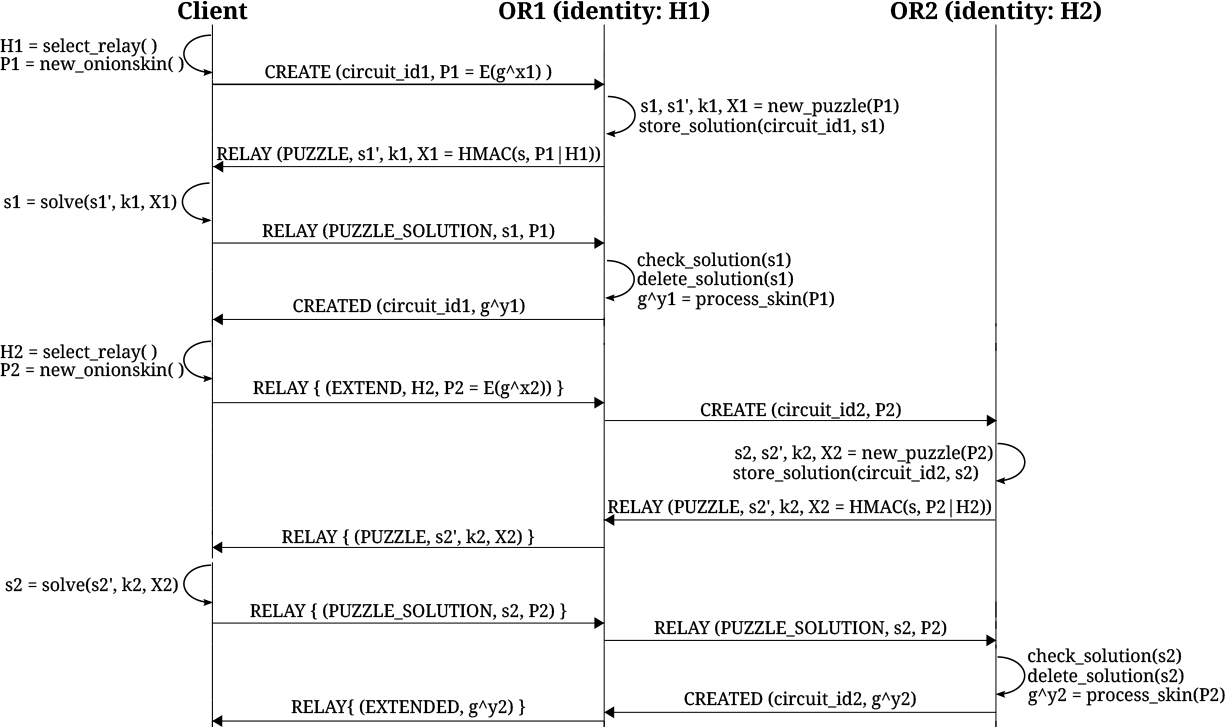
\includegraphics[width=0.95\textwidth]{./figure//clientpuzzles}
\caption{Funzionamento dei client puzzles.}
\label{FIG:ClientPuzzles}
\end{figure}
Una volta che il puzzle viene inviato al client, esso deve risolverlo cercando di indovinare il valore degli ultimi $k$ bit di $s$, che deve per forza essere fatto per tentativi. Per ogni tentativo deve provare una combinazione $s''$, calcolare la funzione $X'$=HMAC($s'', P|H$) e verificare se $X'=X$. Quando l'uguaglianza � verificata, allora ha indovinato il valore di s. Un puzzle di valore $k$ richiede in media $2^{k-1}$ tentativi, e il tempo di calcolo cresce esponenzialmente con k. Questo permette di poter decidere se far lavorare il client pochi millisecondi fino ad arrivare a qualche ora.

Per scambiare i puzzles e le rispettive soluzioni, il client e il router inseriscono nel payload di una {\ttfamily RELAY} cell i comandi {\ttfamily PUZZLE} e {\ttfamily PUZZLE\textunderscore SOLUTION}. Come descritto nelle specifiche di Tor, esse vengono crittografate con le chiavi di sessione precedentemente negoziate, quindi l'unico router che pu� intercettare sia il puzzle che la sua soluzione � l'ultimo tra quelli che fanno parte del circuito gi� creato; nel caso della figura~\ref{FIG:ClientPuzzles} ad esempio, questo � l'$OR1$, nel momento in cui si vuole estendere il circuito fino a l'$OR2$. 
%\underline{L'OR1 per� non pu� interferire con il protocollo, dal momento che \dots}
Come si pu� vedere dalla Figura~\ref{FIG:ClientPuzzles} la sequenza delle operazioni necessarie ad aggiungere un nuovo router al circuito sono le seguenti:
\begin{enumerate}
\item Il client invia una {\ttfamily CREATE} o una  {\ttfamily RELAY\textunderscore EXTEND} cell per selezionare il nuovo router;
\item il router crea il puzzle, memorizza la soluzione e risponde con una {\ttfamily RELAY} cell inserendolo all'interno del payload;
\item il client risolve il puzzle e sempre tramite una {\ttfamily RELAY} cell comunica la soluzione attraverso il comando {\ttfamily PUZZLE\textunderscore SOLUTION};
\item il router controlla se la soluzione $s$ � corretta e in caso affermativo comunica tramite una {\ttfamily CREATED} cell che la connessione � stata stabilita.
\end{enumerate}
%il client richiede di aggiungere un router al path, quindi gli viene inviata una risposta tramite una {\ttfamily RELAY} cell con il puzzle, successivamente deve risolverla e rispondere al router; infine gli viene notificata l'avvenuta connessione.
Memorizzare la soluzione di un puzzle, richiede 18 bytes di memoria (8 per la soluzione del puzzle, 8 per l'ID della connessione e 2 per l'ID del circuito). Quindi un potenziale aggressore potrebbe sfruttare questa piccola occupazione di memoria per condurre un attacco che tenta di consumare la RAM libera del router facendo molte richieste ad esso e lasciando i puzzle irrisolti. Per fare in modo che questo non accada, viene assegnata una scadenza $\Delta_{p}$ al puzzle, entro il quale deve essere risolto, altrimenti la soluzione viene eliminata dalla memoria. Scegliere un $\Delta_{p}$ adeguato non � difficile, in quanto anche scegliendolo pari a 2 minuti un aggressore che ha a disposizione un bitrate di 189 Mbit/s riesce a consumare solo 100 MB di memoria. Inoltre � stato verificato che la rete Tor supporta uno stream di {\ttfamily CREATE} cell di pochi Mbit/s. Un $\Delta_{p}$ pari a 2 minuti risulta essere adeguato anche per i client pi� lenti, che riusciranno quindi a risolvere il puzzle in tempo. Inoltre il valore di $\Delta_{p}$ pu� essere modificato a seconda della situazione. Una strategia alternativa potrebbe essere quella di scegliere una sola chiave $s$ che dopo un certo periodo di tempo viene sostituita, in modo da evitare che un aggressore possa utilizzarla pi� volte. Questo permette di memorizzare solo una soluzione, ma scegliere il periodo di scadenza � un'operazione difficile che richiede una stima accurata del bitrate a disposizione dell'aggressore e della velocit� con cui i client benigni riescono a risolvere il puzzle. Un valore troppo grande rischia di essere pericoloso, mentre troppo piccolo svantaggia i client onesti.

\subsubsection{Scelta della difficolt� del puzzle}
Si possono seguire due approcci differenti nell'implementazione dei client puzzle: inviarli ai client, in qualunque situazione con un livello di difficolt� fissata oppure inviarli solo se il router diventa obiettivo di un attacco. Il primo approccio � pi� facile da implementare ma richiede risorse inutili ai client benigni, mentre il secondo non comporta l'utilizzo di risorse inutili ma per essere efficace bisogna essere in grado di capire se il router sta subendo un attacco DoS. Per capire se l'OR � sotto attacco, si pu� pensare di contare ogni $\Delta_{x}$ secondi il numero $P_{x}$ di {\ttfamily CREATE} cell che � stato in grado di processare e il numero $D_{x}$ che invece sono state scartate dato che i CPU workers erano occupati. � possibile quindi calcolare il valore $\overline{\mu}=\frac{D_{x}}{P_{x}}$ e controllare ogni $\Delta_{x}$ secondi se la percentuale di richieste scartate sta sopra o sotto una certa soglia $\beta$. La prima volta che $\overline{\mu}$ supera il valore di soglia $\beta$, il router inizia ad inviare i puzzle a tutti i client che desiderano aggiungerlo al proprio circuito, con una difficolt� iniziale di parametro $k$ (i.e. $k=16$) per $\Delta_{x}$ secondi. Alla fine dell'intervallo l'$OR$ aumenta di 1 il valore di $k$ se $\overline{\mu}>\beta$, mentre lo diminuisce di 1 se $\overline{\mu}<\beta$; questo permette di variare dinamicamente la difficolt� del puzzle. Per evitare invece di assegnare un carico di lavoro troppo elevato ai client onesti, si pu� fissare un limite per $k$ (ad esempio 20). Il parametro $\beta$ dovrebbe essere fissato ad un valore basso, molto vicino allo 0. La scelta va fatta tenendo conto di quante cell i CPU workers potrebbero scartare durante una situazione di normalit�. Infine il valore di $\Delta_{x}$ non � critico, basta che permetta di scegliere la difficolt� dell puzzle correttamente.

\section{Sniper Attack}
Lo \emph{Sniper Attack} � potenzialmente uno degli attacchi DoS pi� distruttivi ed efficaci, infatti \emph{permette anonimamente di disabilitare qualsiasi nodo Tor utilizzando pochissime risorse}. L'attacco pu� essere anche usato per identificare un servizio nascosto, mediante la disabilitazione selettiva dei relay. Esso si basa sul livello di congestione e sul meccanismo di controllo del traffico di Tor per causare un aumento incontrollato del contenuto del buffer dell'obiettivo. L'idea di base � quella di costruire un normale circuito Tor, utilizzando il nodo da colpire come entry e iniziare a scaricare  un file di grosse dimensioni. Contemporaneamente si smette di leggere dal buffer in input e si invia con una certa frequenza il comando {\ttfamily SENDME} al nodo di uscita, per costringerlo ad immettere dati nel circuito. La procedura pu� essere ripetuta per vari circuiti, utilizzando sempre l'obiettivo come nodo d'ingresso. Quando la memoria del nodo sar� esaurita, il processo Tor verr� terminato dal sistema operativo del nodo, causandone l'inoperabilit�. Secondo gli studi di \cite{sniper}, un attacco di questo tipo sarebbe in grado, in soli 29 minuti, di disabilitare i 20 pi� importanti nodi di uscita di tutta la rete; tutto questo inoltre con un costo bassissimo per chi conduce l'attacco. Infatti � possibile costringere l'obiettivo a consumare fino a 2187 KiB/s di memoria utilizzando un bitrate di solo 92 KiB/s in upstream e 39 KiB/s in downstream.

Per capire a fondo l'attacco per�, � necessario prima conoscere come Tor gestisce il traffico nel circuito. Tor implementa un meccanismo a  finestra variabile per controllare la quantit� di dati che viene immessa nella rete. Ogni nodo estremo del circuito (i.e. client ed exit) tiene traccia con due contatori di due finestre. Il \emph{package} window, inizializzato al valore 1000, controlla quante data cell un $OR$ � autorizzato a "impacchettare" e inserire all'interno del circuito, mentre il \emph{delivery} window, inizializzato al valore 100, quante data cell � disposto a consegnare al di fuori di esso. Il primo contatore viene decrementato di uno quando una data cell viene \emph{inserita} all'interno del circuito, mentre il secondo per ogni data cell che viene \emph{rimossa}. Per ogni circuito possono esistere pi� stream: in questo caso si dice che gli stream sono multiplati; i circuiti invece sono multiplati sulle connessioni. Analoghi contatori esistono per ogni stream, quindi avremo un \emph{package} window, questo inizializzato a 500, e un \emph{delivery} window, inizializzato a 50. Il packaging edge (PE) di un circuito smette di introdurre data cell da uno qualsiasi degli stream multiplati il cui package window raggiunge il valore zero, oppure interrompe tutti i flussi di data cell di tutti gli stream quando il package window del circuito va a zero. Il delivery edge (DE) manda un comando di feedback chiamato {\ttfamily SENDME} al PE quando la delivery window di un circuito o quella di uno stream raggiungono il valore zero. Questo comando riporta il valore del delivery window del DE e del package window del PE al loro rispettivo valore iniziale\footnote{In pratica il package window di circuito e di stream sono inizializzati rispettivamente a 1000 e a 500, mentre i delivery window a 100 e 50. Quando il PE invia una cell verso il DE, vengono decrementate di 1 sia i delivery window del DE che i package window del PE (sia dello stream corrispondente che del circuito). Normalmente, proseguendo in questo modo, il delivery window di uno degli stream o quello del circuito raggiunger� il valore zero. Questo significa che il package window dello stream avr� valore 450 oppure che il delivery window del circuito avr� valore 900. Il segnale di {\ttfamily SENDME} riporter� i valori dei delivery window a 100 e a 50, mentre quelli dei package window a 1000 e a 500.}. Quindi per un dato stream non ci saranno pi� di 500 data cell all'interno della rete, e non pi� di 1000 per un singolo circuito.
\subsubsection{Attacco basilare}
Un DE che smette di leggere dal buffer di una connessione causa l'accodamento di un intera package window proveniente da un PE (1000 cell), assumendo che per ogni circuito attivo ci siano almeno due stream multiplati e che la quantit� di dati che viene trasferita sia sufficiente a portare il package window del PE a zero.

\begin{figure}[!htbp]
\centering
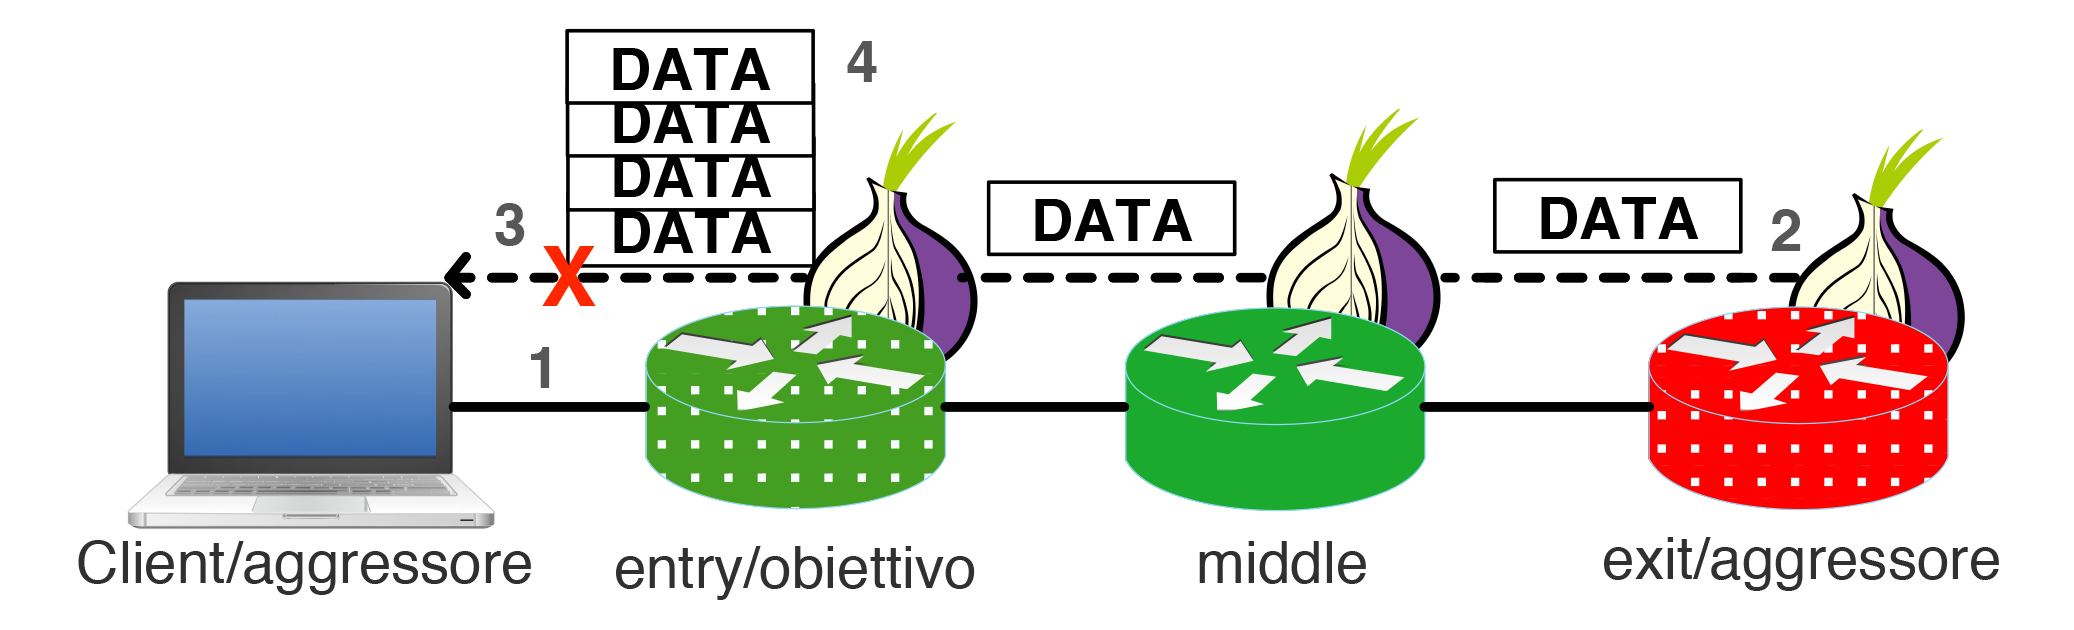
\includegraphics[width=0.7\textwidth]{./figure//attaccobase}
\caption{Sniper Attack basilare.}
\label{FIG:BaseAttack}
\end{figure}

L'attacco si compone quindi delle seguenti fasi:
\begin{enumerate}
\item Il client costruisce un circuito selezionando l'obiettivo come entry e un relay complice come exit;
\item Il nodo di uscita genera pacchetti e li invia al client attraverso il circuito, ignorando il limite del package window;
\item Il client smette di leggere dalla connessione TCP stabilita con l'obiettivo;
\item Il buffer dell'obiettivo inizia a riempirsi fino a quando il sistema operativo non termina il processo Tor.
\end{enumerate}
Una piccola variante dell'attacco appena descritto consiste nell'utilizzare un file server come complice. In questo caso � il client a generare una grande quantit� di dati da inviare al server che contemporaneamente smetter� di leggere dal buffer TCP, causando il riempimento della memoria e conseguentemente la terminazione del processo dell'exit router. Con questa variante dell'attacco � quindi possibile colpire un exit router.

%\begin{figure}[!htbp]
%\centering
%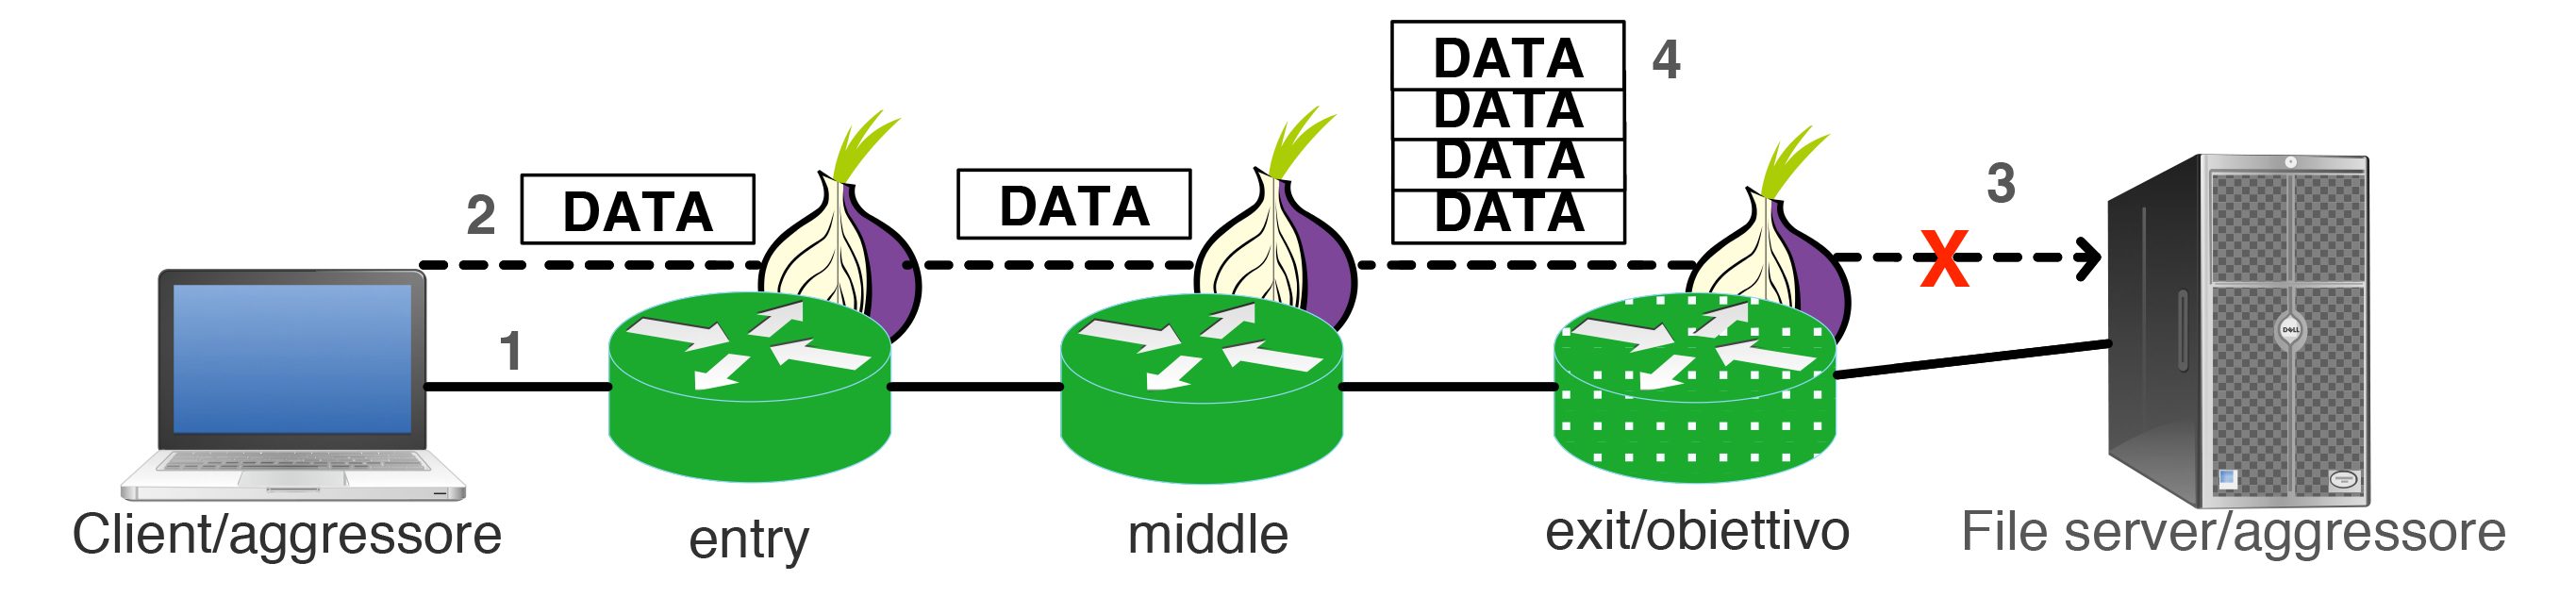
\includegraphics[width=0.7\textwidth]{./figure//variante}
%\caption{Variante Sniper Attack.}
%\label{FIG:VariantAttack}
%\end{figure}

Da notare il fatto che con \emph{entrambe} le varianti si pu� colpire anche un \emph{middle} router: nella prima versione � sufficiente avere come complice un entry relay che smette di leggere dal buffer della connessione con il middle router; nella seconda basta un exit relay che anch'esso smette di leggere dal buffer TCP.

\subsection{Attacco avanzato}

\begin{figure}[!htbp]
\centering
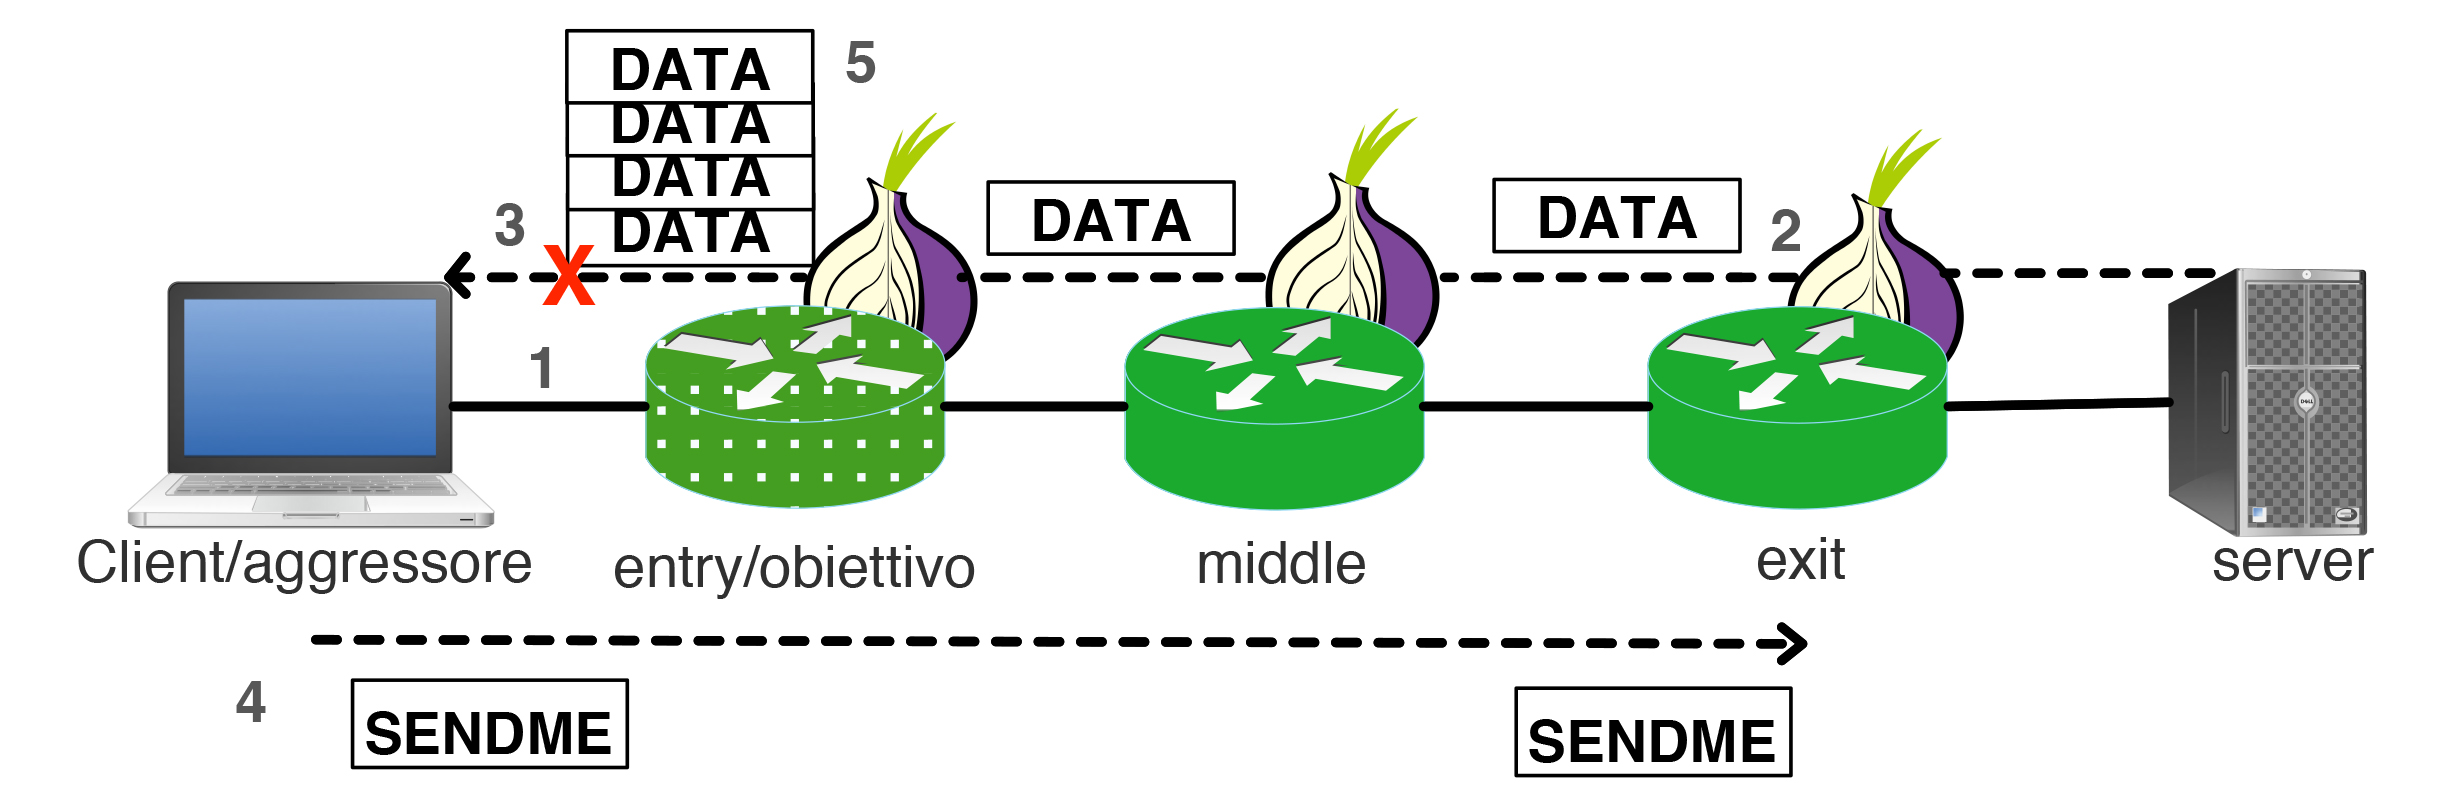
\includegraphics[width=0.7\textwidth]{./figure//sniperattack-advance+sendme}
\caption{Sniper Attack avanzato.}
\label{FIG:SniperAttackAdv }
\end{figure}

L'attacco avanzato non necessita di un router/server complice e si basa su:
\begin{itemize}
\item interruzione della lettura dalla connessione TCP;
\item utilizzo del comando {\ttfamily SENDME}.
\end{itemize}
Per prima cosa il client-aggressore (DE) deve stabilire un circuito, selezionando come entry router l'obiettivo da colpire. Successivamente deve iniziare a scaricare un file di grandi dimensioni.
Una volta che il client smette di leggere dalla connessione stabilita con l'obiettivo, inizia ad inviare il comando {\ttfamily SENDME} al nodo di uscita (PE), in modo da evitare che la package window raggiunga il valore zero, smettendo cos� di immettere pacchetti nel circuito.
Tor per� possiede un meccanismo di protezione contro i client che provano ad inviare continuamente il comando {\ttfamily SENDME} per ottenere pacchetti con una maggiore frequenza: quando un exit riceve un {\ttfamily SENDME} che tenta di far alzare il valore della package window sopra a quello iniziale (1000), si accorge della violazione, chiude il circuito e invia un {\ttfamily DESTROY} al nodo precedente che lo inoltra all'entry e poi al client. Quando il client riceve il comando {\ttfamily DESTROY}, chiude anch'esso il circuito e lo inoltra all'entry e al middle che fanno la stessa cosa. Se questo accade, l'obiettivo, chiudendo il circuito, svuota il buffer e quindi l'attacco non va a buon fine. Per condurlo con successo bisognerebbe evitare che il contatore package window del nodo di uscita superasse la soglia iniziale, e che il client non inviasse il comando di eliminazione del circuito. Solo la seconda condizione si verifica dato che il client non legger� dalla connessione con l'entry relay e quindi non ricever�, n� inoltrer� il comando {\ttfamily DESTROY}. Bisogna quindi inviare il comando {\ttfamily SENDME} con una frequenza n� troppo alta, che causa l'eccedere del package window, n� troppo bassa che rende inefficace l'attacco.  Per calcolare ogni quanto inviare il {\ttfamily SENDME} al nodo di uscita � sufficiente stimare il throughput $S$ della connessione scaricando un file di una certa dimensione. Se vengono trasferiti $\sigma$ KiB in $\Delta$ secondi allora $S=\frac{\sigma}{\Delta}$ KiB/s o anche $S=\frac{2\sigma}{\Delta}$ cells/s, dato che una cell Tor � di 512 byte.
Il comando va inviato ogni 50 cell ricevute a livello di stream e ogni 100 ricevute a livello di circuito, ma senza leggere dalla connessione � impossibile contarle. Con le stime del throughput � possibile per� sapere ogni quanti secondi inviare il comando: $T_{ss}=\frac{25 \Delta}{\sigma}$ e $T_{cs}=\frac{50 \Delta}{\sigma}$.
%questi i periodi di invio rispettivamente. � necessario conoscere i periodi con cui inviare il comando dato che non leggendo dal buffer di input � impossibile sapere quanti cell sono state ricevuti.

Dato che il throughput della connessione � un parametro che pu� variare facilmente, � possibile che il client invii troppo frequentemente il {\ttfamily SENDME}, causando l'avvio del meccanismo di protezione. Questo, anche se non provoca lo svuotamento del buffer dell'entry/obiettivo, non permette pi� di utilizzare quel circuito per condurre l'attacco. Per risolvere questo problema e per diminuire il tempo necessario a riempire il buffer dell'entry � possibile parallelizzare l'azione offensiva. Per fare ci� si possono utilizzare \emph{team} di circuiti, ad ognuno dei quali � assegnato un path Tor. Per ogni team uno dei circuiti si occuper� di stimare il throughput, mentre gli altri di inviare il comando {\ttfamily SENDME}, utilizzando due processi Tor separati per team che svolgono le due funzioni. Infine, dato che non si hanno informazioni sullo stato dei circuiti creati, � possibile crearne di nuovi per assicurarsi che il consumo di memoria dell'obiettivo continui regolarmente.

Manca un altro aspetto da trattare (forse il pi� importante di tutti): mantenere l'anonimato. Condurre l'attacco senza essere scoperti � una delle cose pi� importanti e Tor pu� essere utile in questo. Un modo, detto \emph{diretto} � quello di usare un exit node come aggressore, ovvero essere in questa situazione: $\mathcal{E}_A \mathcal{C}_A \leftrightarrow \mathcal{G}_O \leftrightarrow \mathcal{M} \leftrightarrow \mathcal{E} \leftrightarrow \mathcal{S}$ dove $\mathcal{E}$ indica un nodo di uscita, $\mathcal{G}_O $ un nodo d'ingresso (obiettivo), $\mathcal{M}$ un middle, e $\mathcal{S}$ un server. Un obiettivo non � in grado di capire se il nodo di uscita � il responsabile dell'attacco o se sta solo operando come servitore.
Lo svantaggio � che l'exit node, per essere tale, deve mettere a disposizione una certa quantit� di risorse nella rete e quindi alla fine l'attacco ne richiederebbe pi� di quante effettivamente necessarie. Inoltre, dato che l'obiettivo sarebbe direttamente connesso con l'aggressore, conoscerebbe il suo indirizzo IP, che potrebbe essere utilizzato per rintracciarlo e localizzarlo. Alternativamente si pu� pensare di utilizzare un intero circuito per nascondere l'IP. Questa tipologia di attacco viene detta \emph{anonima}. Ci si troverebbe quindi in questa situazione: $\mathcal{C}_A^2 \mathcal{C}_A^1 \leftrightarrow \mathcal{G} ^1\leftrightarrow \mathcal{M}^1 \leftrightarrow \mathcal{E}^1 \leftrightarrow \mathcal{G}_{O}^2 \leftrightarrow \mathcal{M}^2 \leftrightarrow \mathcal{E}^2 \leftrightarrow \mathcal{S}$ dove "1" indica il circuito di ingresso nella rete e "2" il circuito vero e proprio dell'attacco. $\mathcal{C}_A^1$ smette di leggere dalla connessione, mentre $\mathcal{C}_A^2$ invia il comando {\ttfamily SENDME}. In una configurazione di questo tipo potrebbe essere difficile stimare il throughput della connessione, inoltre due circuiti creati in sequenza potrebbero far nascere dei sospetti.

Dato che i top 100 relay, secondo il bitrate, vengono selezionati con una probabilit� del 40\%, un attacco che colpisce anche un piccolo numero di questi ultimi ha un impatto significativo sulle prestazioni della rete. Sono state fatte delle simulazioni \cite{sniper} su uno scenario reale e sono stati misurati i tempi impiegati a disabilitare alcune categorie significative di nodi/infrastrutture Tor. � stato valutato sia l'effetto di un attacco diretto, sia anonimo, ciascuno su macchine con 1GiB e 8 GiB di RAM. L'analisi mostra che con l'attacco diretto � possibile disabilitare in solo un minuto il top {\ttfamily FAST}\footnote{{\ttfamily FAST} � un flag assegnato dalle directory authorities ad un router che indica che esso � adatto a costruire circuiti con un bitrate elevato. \cite{torspec}} Guard e il top {\ttfamily FAST} Exit con 1GiB di RAM, mentre con 8 GiB di RAM i tempi diventano rispettivamente di 18 e 8 minuti. Inoltre in soli 29 minuti � possibile escludere i top 20 Exit, causando problemi al 35\% dei path costruiti in tutta la rete.

\begin{table}[]
\centering
\caption{Simulazione Sniper Attack}
\label{Tab:sniperattack}
\begin{tabular}{cccccc}
\multicolumn{1}{l}{}                    & \multicolumn{5}{c}{Tempo in H:M per consumare tutta la RAM}                                                                                       \\ \cline{3-6} 
                                        & \multicolumn{1}{c|}{}       & \multicolumn{2}{c|}{Diretto}                              & \multicolumn{2}{c|}{Anonimo}                           \\ \cline{2-6} 
\multicolumn{1}{c|}{}                   & \multicolumn{1}{c|}{Sel \%} & \multicolumn{1}{c|}{1 GiB} & \multicolumn{1}{c|}{8 GiB}  & \multicolumn{1}{c|}{1 GiB} & \multicolumn{1}{c|}{8 GiB}  \\ \hline
\multicolumn{1}{|c|}{Top {\ttfamily FAST} Guard}    & \multicolumn{1}{c|}{1.7}    & \multicolumn{1}{c|}{0:01}  & \multicolumn{1}{c|}{0:18}   & \multicolumn{1}{c|}{0:02}  & \multicolumn{1}{c|}{0:14}   \\
\multicolumn{1}{|c|}{Median {\ttfamily FAST} Guard} & \multicolumn{1}{c|}{0.025}  & \multicolumn{1}{c|}{0:23}  & \multicolumn{1}{c|}{3:07}   & \multicolumn{1}{c|}{0:23}  & \multicolumn{1}{c|}{3:07}   \\
\multicolumn{1}{|c|}{Bottom {\ttfamily FAST} Guard} & \multicolumn{1}{c|}{1.9e-4} & \multicolumn{1}{c|}{1:45}  & \multicolumn{1}{c|}{14:03}  & \multicolumn{1}{c|}{1:45}  & \multicolumn{1}{c|}{13:58}  \\ \hline
\multicolumn{1}{|c|}{Top {\ttfamily FAST} Exit}     & \multicolumn{1}{c|}{3.2}    & \multicolumn{1}{c|}{0:01}  & \multicolumn{1}{c|}{0:08}   & \multicolumn{1}{c|}{0:01}  & \multicolumn{1}{c|}{0:12}   \\
\multicolumn{1}{|c|}{Median {\ttfamily FAST} Exit}  & \multicolumn{1}{c|}{0.01}   & \multicolumn{1}{c|}{1:45}  & \multicolumn{1}{c|}{14:03}  & \multicolumn{1}{c|}{1:22}  & \multicolumn{1}{c|}{10:53}  \\
\multicolumn{1}{|c|}{Bottom {\ttfamily FAST} Exit}  & \multicolumn{1}{c|}{6e-5}   & \multicolumn{1}{c|}{1:45}  & \multicolumn{1}{c|}{14:03}  & \multicolumn{1}{c|}{1:48}  & \multicolumn{1}{c|}{14:20}  \\ \hline
\multicolumn{1}{|c|}{Top 5 Guards}      & \multicolumn{1}{c|}{6.5}    & \multicolumn{1}{c|}{0:08}  & \multicolumn{1}{c|}{1:03}   & \multicolumn{1}{c|}{0:12}  & \multicolumn{1}{c|}{1:37}   \\
\multicolumn{1}{|c|}{Top 20 Guards}     & \multicolumn{1}{c|}{19}     & \multicolumn{1}{c|}{0:45}  & \multicolumn{1}{c|}{5:58}   & \multicolumn{1}{c|}{1:07}  & \multicolumn{1}{c|}{8:56}   \\ \hline
\multicolumn{1}{|c|}{Top 5 Exits}       & \multicolumn{1}{c|}{13}     & \multicolumn{1}{c|}{0:05}  & \multicolumn{1}{c|}{0:37}   & \multicolumn{1}{c|}{0:07}  & \multicolumn{1}{c|}{0:57}   \\
\multicolumn{1}{|c|}{Top 20 Exits}      & \multicolumn{1}{c|}{35}     & \multicolumn{1}{c|}{0:29}  & \multicolumn{1}{c|}{3:50}   & \multicolumn{1}{c|}{0:44}  & \multicolumn{1}{c|}{5:52}   \\ \hline
\multicolumn{1}{|c|}{All Dir Auths}     & \multicolumn{1}{c|}{N/A}    & \multicolumn{1}{c|}{17:34} & \multicolumn{1}{c|}{140:32} & \multicolumn{1}{c|}{17:44} & \multicolumn{1}{c|}{141:49} \\ \hline
\end{tabular}
\end{table}

\subsection{Difesa contro lo Sniper Attack}
Lo Sniper Attack sfrutta principalmente due problemi intrinseci di Tor: mancanza di un controllo di flusso e assenza di bound e check sulle code attive. Questi problemi possono essere risolti con delle tecniche che verranno discusse in seguito.

\subsubsection{{\ttfamily SENDME} autenticati}
Nelle sezioni precedenti � stato mostrato come i packaging edge non sono in grado di verificare che i delivery edge abbiano ricevuto le cell. Ogni packaged cell contiene un hash del suo contenuto cos� da permettere al client di rilevare degli errori sui bit. Si potrebbe fare in modo che un package edge richieda gli hash di ogni packaged cell nel comando {\ttfamily SENDME}, anche se un malintenzionato potrebbe scaricare un file di cui aveva precedentemente calcolato gli hash durante l'attacco cos� da aggirare il controllo. Per fare in modo che questo non accada il PE potrebbe inserire un byte casuale ogni 100 cell il cui hash dovrebbe essere calcolato e comunicato dal DE. La probabilit� di indovinare il byte e quindi l'hash sarebbe di $1/256 \approx 0.39$ \%. Questo metodo impedisce di avere pi� di 1000 cell contemporaneamente nel circuito e fornisce difesa contro l'attacco avanzato, anche se non evita totalmente i suoi effetti dato che ogni circuito con 1000 cell consuma 500 KiB. Inoltre non difende dall'attacco basilare dove sia il client che l'exit sono sotto il controllo del malintenzionato.

\subsubsection{Bound sulla dimensione delle code}
Prima di continuare � necessario specificare che Tor, per come � stato progettato, crea una coda per ogni circuito, gestita con una pura politica FIFO. Un unico servitore a turno sceglie una coda e inoltra delle cell. \\
Il secondo problema critico � quello della dimensione che le code del processo Tor possono assumere. Esse possono crescere indefinitamente senza nessun controllo. Il metodo pi� semplice per risolvere il problema � quello di impostare un limite sulla dimensione della coda; quando viene superato, il router riconosce una violazione del protocollo e chiude il circuito, impedendo che l'aggressore consumi tutta la memoria. Bisogna per� trovare un limite adeguato: si potrebbe utilizzare un valore intorno al 1000 con delle tolleranze, dato che il numero di cell in transito non possono essere pi� di 1000. Comunque il bound sulla dimensione delle code, come i {\ttfamily SENDME} autenticati non difendono dagli attacchi paralleli, che quindi sarebbero ancora potenzialmente in grado di mandare in crash il processo Tor di un $OR$.

\subsubsection{Eliminazione adattiva circuito}
Per superare le limitazioni dei metodi precedenti, � stato sviluppato un altro meccanismo molto pi� sicuro. L'approccio utilizzato � quello di continuare a chiudere circuiti attivi fintanto che il \emph{totale} della memoria utilizzata rimane sopra una certa soglia; il nuovo problema diventa quindi decidere quale circuito chiudere. Chiudendo il circuito con la coda pi� lunga un aggressore potrebbe creare molti circuiti con code brevi, causando l'eliminazione di quelli che non fanno parte dell'attacco ma di traffico ordinario. Gli autori \cite{sniper} quindi propongono di eliminare il circuito con la cell pi� vecchia in testa alla propria coda; � necessario quindi che ogni cell sia etichettata con un timestamp. Dato che ogni coda � gestita con una pura politica FIFO, la cell in testa sar� la pi� vecchia di quel circuito. Per questo un eventuale aggressore sarebbe costretto a leggere continuamente dai propri circuiti per mantenere "giovani" le cell, altrimenti dopo una certa quantit� di tempo verrebbero chiusi. \\ Assumiamo che il bitrate $B$ di un $OR$ sia uguale sia in ingresso che in uscita e che $n$ sia il numero di circuiti attivi sul router in un certo momento. Sarebbe ragionevole pensare che il throughput venga diviso equamente tra tutti i circuiti, ma questo non succede in pratica. Si pu� assumere quindi che ogni circuito abbia a disposizione un throughput di almeno:

\begin{equation}
r\ge \alpha \frac{B}{n}
\end{equation}
con $0<\alpha \le1$.
Ipotizziamo inoltre che esista anche un upper bound sulla coda di dimensione $Q$, diciamo circa di 1000 cell. Osserviamo che se la lunghezza della coda di un circuito benigno non supera il limite $Q$ e il suo rate medio � almeno $r$, allora il massimo tempo che una cell spende nella coda � di:

\begin{equation}
d_{max}=\frac{Q}{r}=\frac{Qn}{\alpha B}.
\end{equation}
Quindi se con $t_{now}$ ci riferiamo all'attuale punto nel tempo, allora le cell in testa alle code dei circuiti benigni devono avere un timestamp pi� grande di $t_{now}-d_{max}$. Un eventuale aggressore dovrebbe fare in modo che le cell non spendano pi� di $d_{max}$ in coda; dovrebbero allora arrivare in un punto del tempo maggiore di $t_{now}-d_{max}$. Solo in questo modo un circuito benigno potrebbe essere chiuso al posto di quello dell'aggressore. Conseguentemente le cell del circuito di attacco devono arrivare ad intervalli di tempo $d$ con $0< d \le d_{max}$. Sia $M$ la quantit� di memoria libera del router prima dell'inizio di un eventuale attacco. L'aggressore dovrebbe riuscire a consumare una quantit� M di memoria per causare l'eliminazione di circuiti benigni. Dato che il tempo che intercorre tra gli arrivi di due cell deve essere al massimo di $d_{max}$, allora il tasso medio minimo con cui l'attaccante deve inviare cell al relay � di:

\begin{equation}
r_a=\frac{M}{d_{max}}=\frac{M}{Q} \cdot \alpha \frac{B}{n}=\frac{M}{Q} \cdot r.
\end{equation}
$M/Q$ � facilmente un numero molto grande vista l'ampia capacit� di memoria delle macchine attuali; chi attacca quindi dovrebbe farsi riservare una grande quantit� di banda dal router per fare in modo che qualche circuito benigno venga chiuso. Anche se un attacco di questo tipo � possibile in teoria, in pratica risulta molto difficile da condurre, principalmente per due motivi:
il primo � che i router servono in modo equo le code dei circuiti, il secondo motivo � che utilizzare quasi tutta la banda del router costituisce da solo un attacco devastante, infatti se l'aggressore disponesse di una larghezza di banda sufficiente a condurre questo tipo di attacco, sceglierebbe un classico attacco DoS che risulterebbe molto pi� efficace.

\begin{figure}[!htbp]
\centering
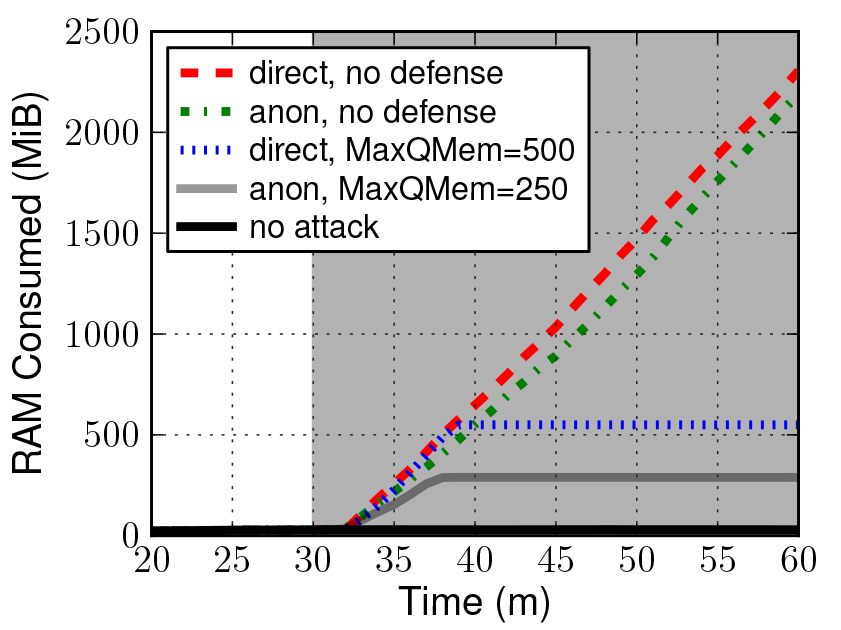
\includegraphics[width=0.5\textwidth]{./figure//sniper}
\caption{Sniper Attack con difesa e senza difesa.}
\label{FIG:SnipDif}
\end{figure}

\subsection{Identificazione di servizi nascosti}
Per riuscire ad individuare un servizio nascosto, un aggressore deve controllare almeno un relay che pu� funzionare da guard e almeno un altro router che serve da rendezvous. Un Onion Router, per poter essere etichettato come guard deve soddisfare un uptime minimo e garantire una certo bitrate; mentre per essere utilizzato come punto di rendezvous non ci sono particolari vincoli da rispettare. L'attacco per identificare un servizio nascosto � suddiviso in tre fasi: 
\begin{enumerate}
\item identificare i guard del servizio nascosto;
\item disabilitare i guard con lo Sniper Attack;
\item controllare se il server che ospita il servizio nascosto ha selezionato un relay controllato come guard sostitutivo. Se questo non si verifica bisogna ripetere la procedura dal punto 1.
\end{enumerate}
Sia $H$ il servizio nascosto, $G_{A}$ il relay controllato dall'aggressore che pu� essere utilizzato come guard, $R_{A}$ il router controllato da usare come punto di rendezvous  e $C_{A}$ il client/aggressore. 

\subsubsection{Fase 1}
Un client pu� fare in modo che $H$ stabilisca nuovi circuiti semplicemente inviandogli delle richieste per fissare l'incontro nel punto di rendezvous $R_{A}$. Ripetendo molte volte questa operazione il server di $H$ sceglier� molto probabilmente (per qualche circuito) il relay controllato $G_{A}$ come middle. In questi casi $G_{A}$ potrebbe potenzialmente sapere quali sono i guard del servizio $H$, ma non riesce a riconoscerli. Per riuscire ad identificarli il router di rendezvous pu� inviare un pattern di 50 {\ttfamily PADDING}\footnote{La {\ttfamily PADDING} cell viene utilizzata per indicare che la connessione � ancora attiva, infatti se non vengono scambiati dati, il client e il router inviano l'un l'altro una cell di questo tipo.} cell ad $H$ seguiti da una {\ttfamily DESTROY} cell. Se $G_{A}$ osserva un pattern di 2 cell da $H$ e di 52\footnote{Le cell in pi� sono quelle utilizzate per la costruzione del circuito.} verso $H$ seguita da una {\ttfamily DESTROY} cell pu� concludere di essere collegato ad un guard di $H$. Utilizzando questa tecnica � possibile, in maniera efficiente, identificare tutti i guard di $H$. Per non creare sospetti � possibile fare le stesse operazioni da $C_{A}$ (al costo di un rate pi� basso) con un normale punto di rendezvous, anzich� utilizzare sempre lo stesso, includendo delle normali richieste dati per farle sembrare delle richieste ordinarie. 

\subsubsection{Fase 2}
Una volta che tutti i guard di $H$ sono stati identificati, essi vengono disabilitati dall'aggressore attraverso lo Sniper Attack. L'attacco pu� essere effettuato in parallelo per ridurre il tempo necessario ad escludere dalla rete gli $OR$; inoltre questo aumenta il tempo in cui tutti i guard sono disabilitati contemporaneamente fornendo un importante vantaggio all'aggressore.

\subsubsection{Fase 3}
Quando tutti i guard sono stati disabilitati, � sufficiente creare delle normali connessioni con $H$ e determinare con una tecnica simile a quella della fase 1 se il router $G_{A}$ � stato scelto come relay d'ingresso nella rete. Se questo si verifica � possibile identificare $H$. 

\subsection{Difesa da attacchi DoS per l'identificazione di servizi nascosti}
L'identificazione di servizi nascosti attraverso la tecnica precedentemente descritta, � un operazione che pu� essere svolta utilizzando qualsiasi attacco DoS da cui la rete Tor � vulnerabile, quindi anche un attacco classico. 
La vulnerabilit� sta nel fatto che un servizio � disposto a scegliere un numero illimitato di entry guard in un certo periodo di tempo; per difendersi quindi � possibile limitare il numero di relay che esso sceglie nei punti cruciali dei propri circuiti, tenendo presente che questo comporta un calo di prestazioni. Inoltre i servizi nascosti rendono troppo semplice l'operazione di identificazione dei guard da parte dell'aggressore, dato che permettono di creare un nuovo circuito ad ogni richiesta di connessione. 

La prima cosa da fare � modificare l'algoritmo con cui vengono scelti gli entry guard. Esso cerca di mantenere un certo numero $a_{g}$ di guard attivi, che corrispondono a quelli che stanno attualmente rispondendo. Inoltre per aumentare la sicurezza fissa un limite $r$ al numero dei guard recenti, cio� che sono stati selezionati meno di $t$ secondi fa. Esso funziona come segue: \emph{se ci sono almeno $a_{g}$ guard attivi ne viene restituito uno a caso; altrimenti se ci sono meno di $r$ guard recenti, seleziona un nuovo guard fino a quando non tornano disponibili $a_{g}$ guard attivi o $r$ guard recenti per poi restituirne uno tra questi; altrimenti se ci sono dei guard attivi ne viene restituito uno casualmente; altrimenti ritorna un errore}. L'algoritmo appena descritto permette di limitare il rate con cui vengono aggiunti nuovi relay della lista dei guard.

La seconda modifica consiste nell'utilizzare dei \emph{middle guard}. Un servizio nascosto $H$ deve mantenere un insieme di middle guard $\mathcal{M}_G$ per ognuno degli entry guard. Ogni volta che $H$ sceglie un guard, poi sceglie casualmente un middle guard da $\mathcal{M}_G$ da usare nel circuito. Questo meccanismo di protezione rende pi� difficile l'individuazione degli entry guard da parte di un potenziale aggressore.

\section{Packet Spinning}
Il \emph{Packet Spinning} \cite{packetspinning}, come gli altri attacchi DoS,
%Il \emph{Packet Spinning} \cite{packetspinning} � un attacco DoS che, come gli altri di questo tipo,%
fa in modo che determinati $OR$ non siano pi� in grado di servire i client che desiderano collegarsi alla rete Tor. Esso utilizza dei loop, dei circuiti artificiali che iniziano e terminano nello stesso punto cos� da tenere occupati una grande quantit� di router alla volta, facendo venire meno la loro capacit� di routing.
Tipicamente un circuito Tor � costituito da tre router: entry, middle ed exit, ma il protocollo non impone vincoli sulla lunghezza del circuito, permettendo quindi di costruirne di pi� lunghi. Fintanto che vengono trasmessi dati, il circuito rimane attivo.
Inoltre Tor � stato progettato in modo che ogni Onion Router non conosca l'intero percorso del circuito, ma solo, chiaramente, i nodi adiacenti.
Il packet spinning si basa su due aspetti fondamentali:
\begin{itemize}
\item i circuiti ad anello sono possibili dato che i router non conoscono l'intero path;
\item un qualsiasi $OR$ spende una certa quantit� di tempo ad effettuare operazioni di tipo crittografico.
\end{itemize}
Per poter condurre l'attacco � necessario che l'aggressore/client abbia anche sotto il proprio controllo un router $R_{c}$. 

Per prima cosa l'aggressore deve creare un circuito che inizi e termini in $R_{c}$ e che passi attraverso tutti gli $OR$ che vuole attaccare. Successivamente il client deve preparare un pacchetto (composto da un certo numero di cell) falso, crittografato livello per livello con le chiavi di sessione negoziate precedentemente e inviarlo al router controllato $R_{c}$ che la inoltrer� al successivo $OR$. Ogni router successivo al primo dovr� decifrare il proprio livello e inoltrare il pacchetto al prossimo (come avviene in una normale sessione). Nel momento in cui il pacchetto raggiunge l'ultimo router e viene inviato ad $R_{c}$ esso lo scarta, reiniettando quello iniziale, crittografato a livelli. Tutta la procedura si pu� ripetere senza limiti di tempo. Inoltre per rendere pi� distruttivo l'attacco � possibile costruire pi� di un loop, combinandoli anche tra di loro, sempre utilizzando $R_{c}$ come nodo di partenza e di arrivo dato che si occupa del mantenimento dell'anello.
Questo attacco risulta particolarmente efficace per tre motivi:
\begin{itemize}
	\item con un solo router controllato � possibile attaccarne pi� di uno;
	\item il router controllato non deve eseguire operazioni crittografiche dato che al termine di ogni giro nell'anello viene reintrodotto il gruppo di cell iniziale;
	\item la differenza tra il carico di lavoro richiesto al router-aggressore e quella degli altri router aumenta all'aumentare di cell utilizzate. 
\end{itemize}


%Questo attacco risulta particolarmente efficace sia perch� attraverso un solo router � possibile tenerne occupati un numero considerevole 
%(idealmente \emph{senza limiti})% 
%e sia perch� il router controllato deve utilizzare molte meno risorse per smistare i pacchetti piuttosto che compiere delle operazioni crittografiche, infatti viene reintrodotto ad ogni giro sempre il gruppo di cell iniziale, . Infine questa differenza cresce con la dimensione del pacchetto iniziale (quindi in base al numero di cell utilizzate). 

\subsection{Rivelazione di comunicazioni anonime}
Una volta che l'aggressore ha utilizzato la tecnica precedentemente descritta, pu� sfruttare questo tipo di attacco per intercettare delle comunicazioni anonime. A questo punto deve utilizzare un gruppo di OR controllati che aveva inserito precedentemente all'interno della rete. Se un client tenta di aggiungere uno dei router sotto attacco per costruire un circuito, molto probabilmente ricever� un timeout dato che sono occupati e non sono in grado di servirlo. Quindi ci sono buone probabilit� che i router controllati verranno scelti al posto di quelli benigni. In questo modo possono essere utilizzate delle altre tecniche, ad esempio di timing analysis \cite{lochidd} per individuare i due interlocutori di una conversazione. 

\begin{figure}[!htbp]
\centering
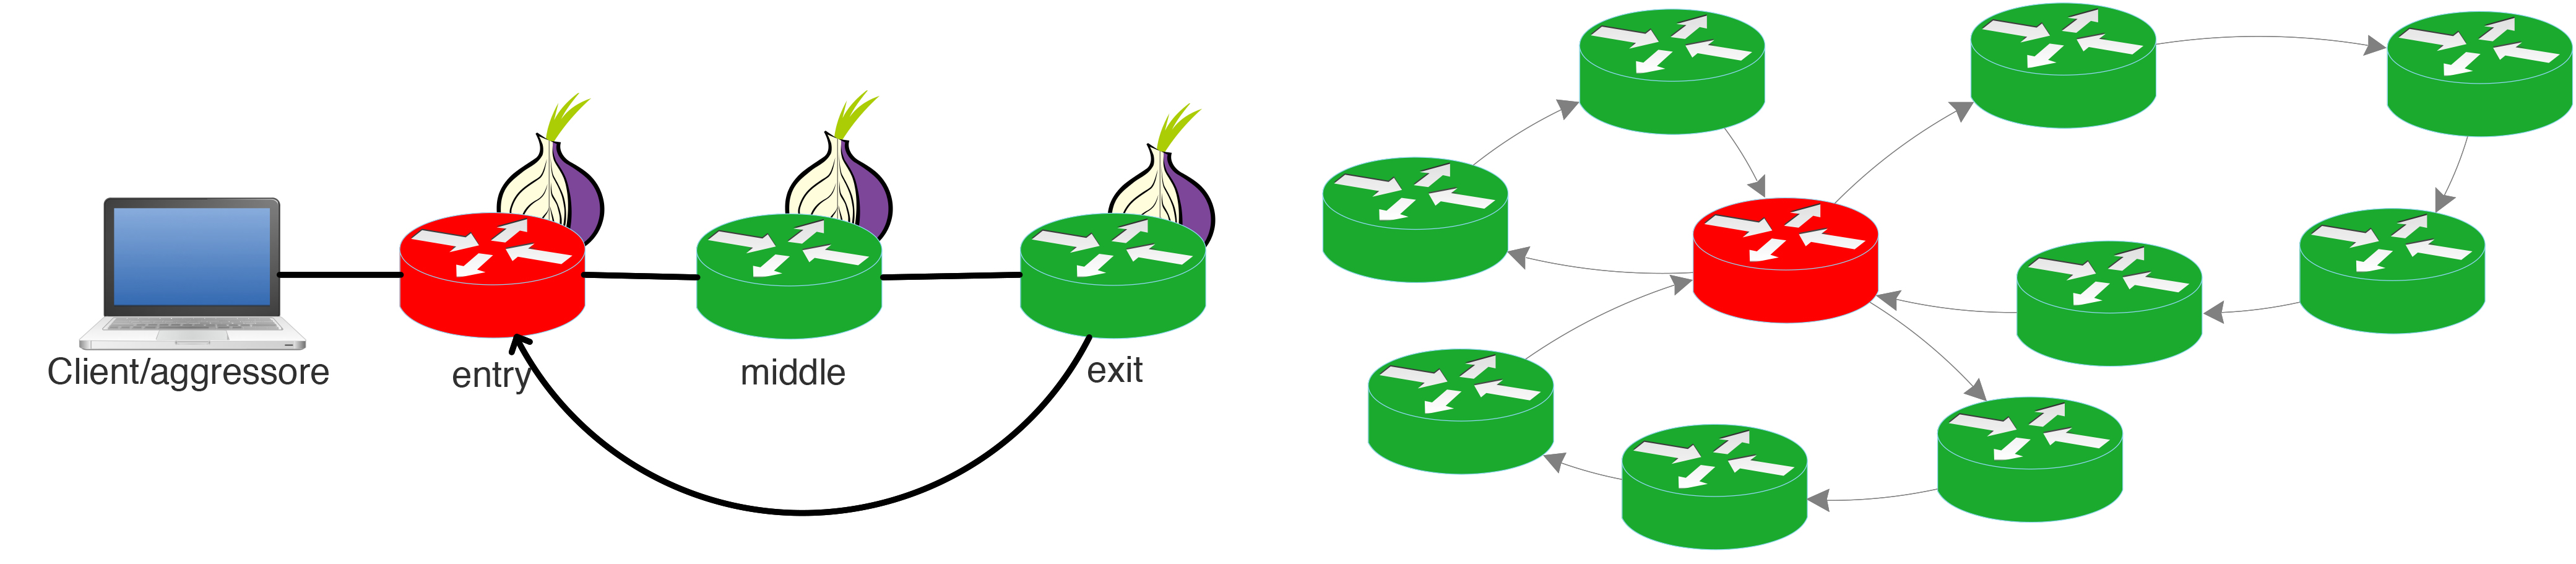
\includegraphics[width=0.95\textwidth]{./figure//packetspinning}
\caption{Loop singolo a sinistra e loop multipilo a destra.}
\label{FIG:PacketSpinning}
\end{figure}

\begin{figure}[!htbp]
\centering
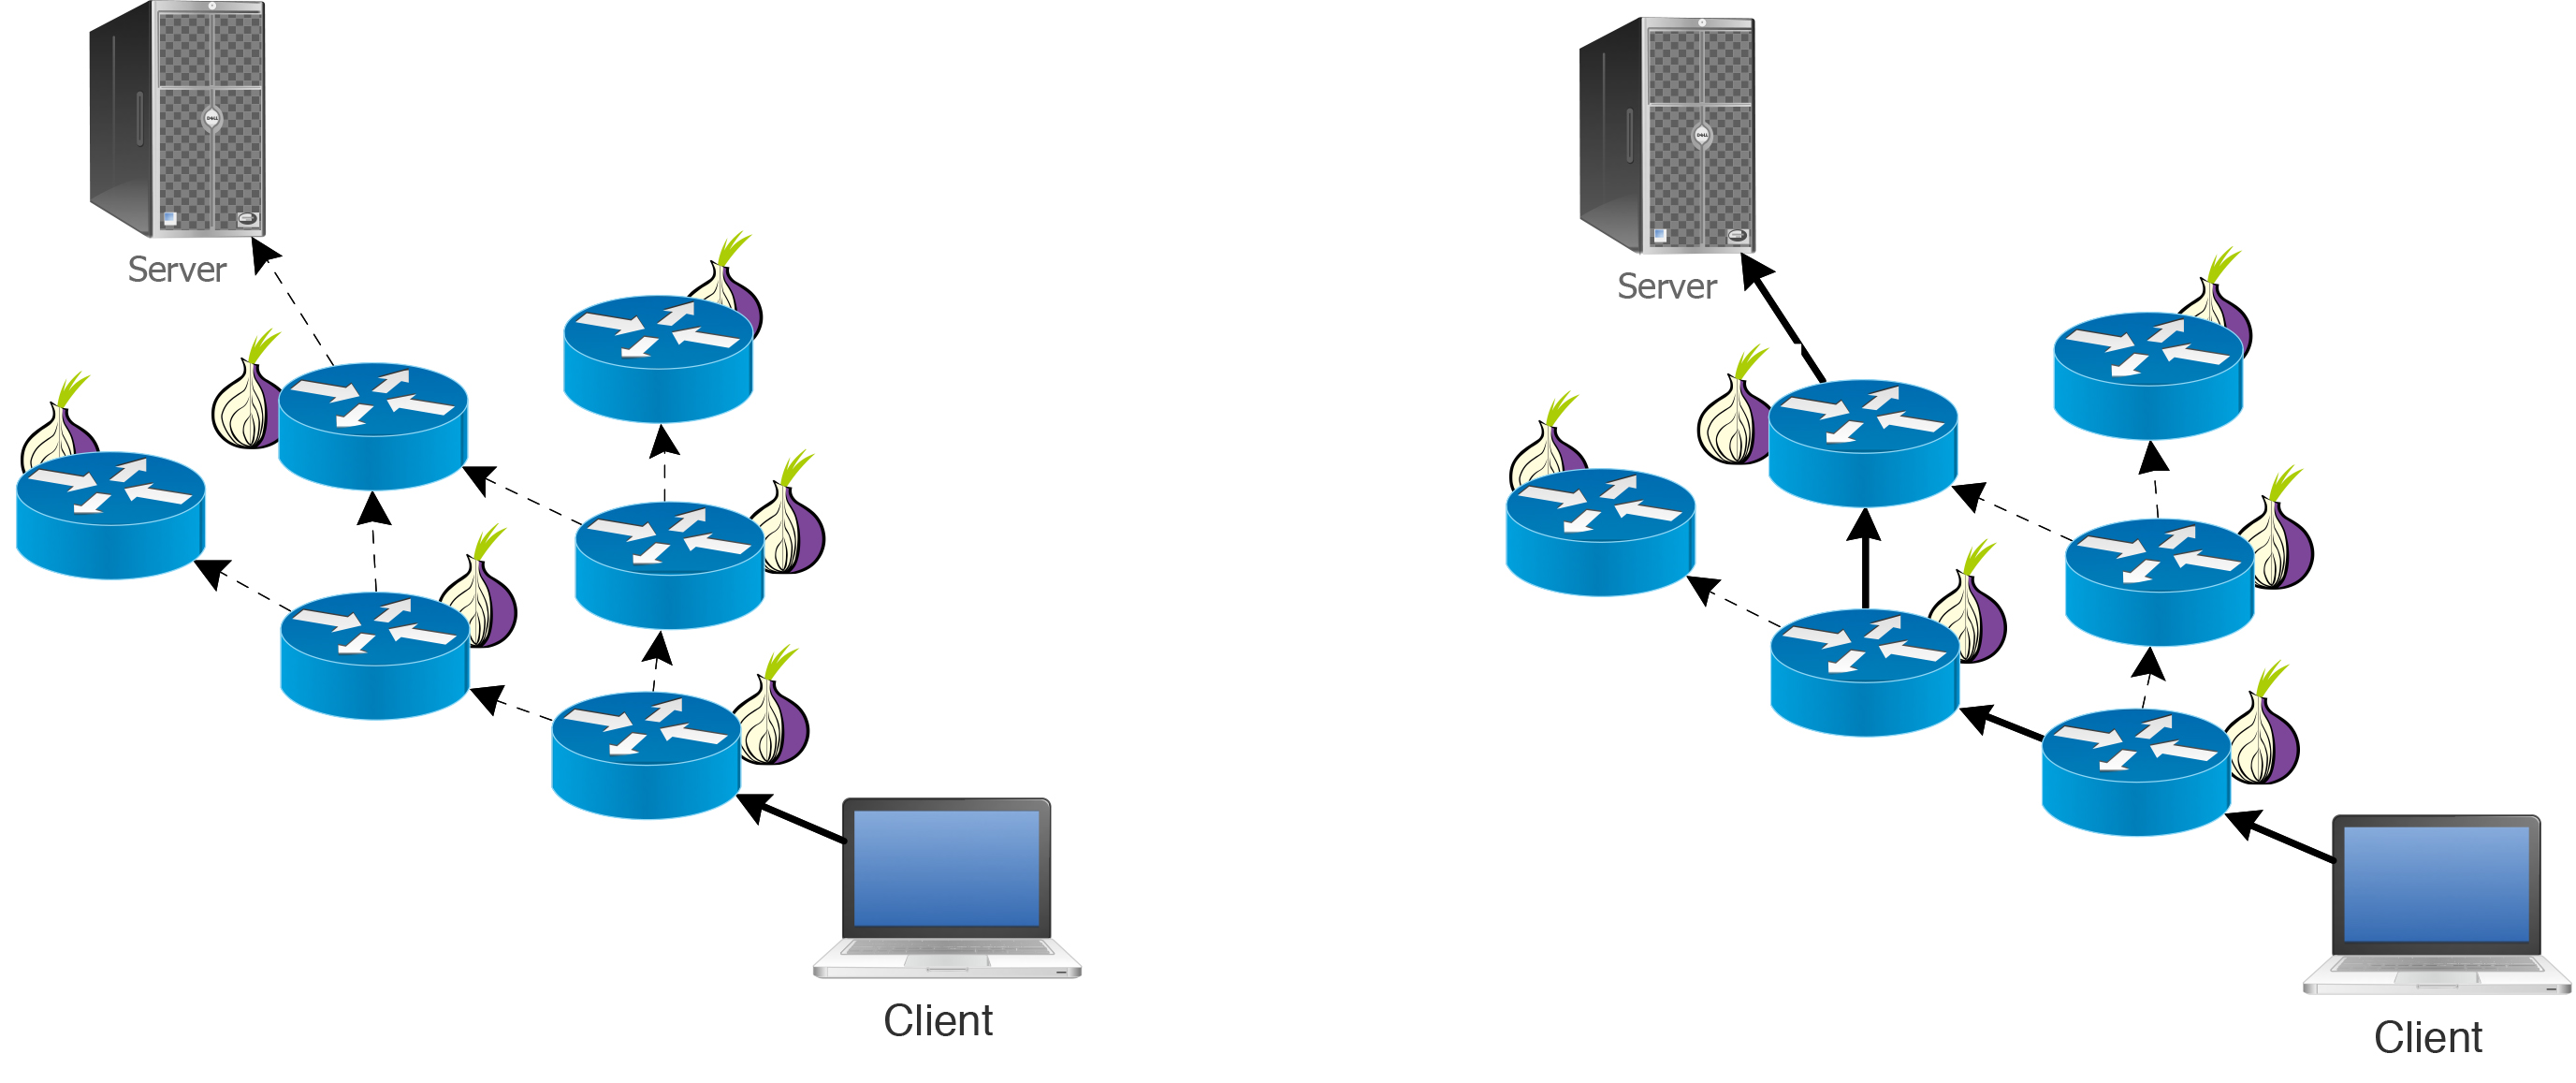
\includegraphics[width=0.95\textwidth]{./figure//TBC}
\caption{TBC, soluzione proposta contro i loop nella rete.}
\label{FIG:tbc}
\end{figure}

\subsection{Difesa attraverso i TBC}
Tor � vulnerabile a questo tipo di attacco perch� permette di costruire dei loop nella rete. Una metodo molto semplice per risolvere questo problema sarebbe quello di fornire delle informazioni sul circuito a tutti i suoi partecipanti. Cos� facendo i router si accorgerebbero che il circuito inizia e finisce nello stesso punto, e non permetterebbero il suo completamento. In questo modo, per�, il livello di anonimato calerebbe drasticamente visto che i router avrebbero delle informazioni sugli altri partecipanti e tutto questo rischierebbe di rendere la rete troppo insicura e vulnerabile.

Gli autori di \cite{packetspinning} propongono di utilizzare i TBC \emph{(Tree Based Circuits)}. Invece di avere un singolo circuito, che si espande telescopicamente dal primo all'ultimo router, � possibile fare in modo di partire dall'entry router, che successivamente stabilir� una connessione con altri due middle router, e ognuno di questi middle router con due exit. Come si pu� vedere anche dalla Figura~\ref{FIG:tbc} i circuiti assumeranno quindi una struttura ad albero. Inoltre durante la costruzione dell'albero alcuni $OR$ posso essere scelti in comune.
Quando si costruiscono circuiti lunghi, il livello di segretezza aumenta, ma allo stesso tempo anche la latenza. Usando i TBC � possibile aumentare il numero di router che si possono utilizzare, senza aumentare la latenza rispetto ad un circuito normale, visto che la profondit� dell'albero pu� rimanere la stessa. Contrariamente ai normali path, i router devono mantenere delle informazioni aggiuntive sul TBC per poter instradare correttamente le richieste. Inoltre una caratteristica fondamentale dei TBC � l'assenza di loop nella rete: ogni volta che viene scambiata una cell i router possono decidere su quale connessione instradarla e quindi questo evita la presenza di anelli. I TBC offrono pi� percorsi alternativi verso la destinazione finale e quindi diminuiscono notevolmente le probabilit� di attraversare router che sono soggetti ad attacchi di packet spinning. Diminuiscono ma non escludono totalmente dato che comunque un aggressore potrebbe avere sotto il proprio controllo uno o pi� router e inoltrare le richieste all'entry in modo da creare dei loop artificiali. 


\clearemptydoublepage

\phantomsection
%\addcontentsline{toc}{chapter}{Considerazioni finali}
\chapter{Conclusioni}


%------------------------------------------------------------------------------------
%Le conclusioni devono essere brevi e comporsi dei seguenti punti:
%\begin{itemize}
%\item indicazione di ci� che si � esposto e del suo significato
%\item analisi comparativa e commento critico dei risultati presentati
%\item spiegazione motivata delle parti omesse o non approfondite
%\item indicazione dei possibili ulteriori sviluppi.
%\end{itemize}
%------------------------------------------------------------------------------------


% ---------------------  ESEMPI UTILI PRONTI ALL'USO  ----------------------------
%TERZO capitolo della tesi. Esempio di citazione doppia \cite{Munoz-Lipo,Vas}.
%
%Esempio di figura in \figurename\ \ref{FIG:LogoUniPD}.
%
%\begin{figure}[!htbp]
%\centering
%
\includegraphics[width=0.25\textwidth]{./figure//LogoUniPD}
%\caption{Esempio di figura.}
%\label{FIG:LogoUniPD}
%\end{figure}
%
%Esempio di tabella in \tablename\ \ref{TAB:Esempio}.
%
%\begin{table}[!htbp]
%\centering
%\renewcommand{\arraystretch}{1.3}
%\caption{Esempio di tabella.}
%\begin{tabular}{cc}
%\hline
%Nome & Valore \\
%\hline
%a & 1 \\
%b & 2 \\
%c & 3 \\
%d & 4 \\
%e & 5 \\
%f & 6 \\
%\hline
%\end{tabular}
%\label{TAB:Esempio}
%\end{table}

%\backmatter

\clearemptydoublepage

%\phantomsection
\addcontentsline{toc}{chapter}{Ringraziamenti}
\chapter*{Ringraziamenti}

Eventuali ringraziamenti personali. % non obbligatorio
%\clearemptydoublepage

\bibliographystyle{IEEEtran}
%\bibliography{IEEEabrv,./7-Bibliografia/Biblio}

\begin{thebibliography}{9} 

\bibitem{tor} R. Dingledine, N. Mathewson, and P. Syverson,\textit{"TOR: The second-generation onion router,"} In USENIX Security Symposium (San Diego, CA, 2004), USENIX Association, pp. 303-320.

\bibitem{tormetrics} Tor Metrics \url{https://metrics.torproject.org/}, [Accesso: 13 Settembre 2016].

\bibitem{torspec} Tor's protocol specifications \url{https://gitweb.torproject.org/torspec.git/tree/dir-spec.txt}, [Accesso: 13 Settembre 2016].

\bibitem{torbridge} Z. Ling, J. Luo, W. Yu, M. Yang, and X. Fu,\textit{"Extensive analysis and large-scale empirical evaluation of Tor bridge discovery,"} in Proc. IEEE INFOCOM, 2012, pp. 2381-2389.

\bibitem{gfc} P. Winter, S. Lindskog, \textit{"How the Great Firewall of China is Blocking Tor,"} Free and Open Communications on the Internet, 2012.

\bibitem{meek} The Tor Project. Meek \url{https://trac.torproject.org/projects/tor/wiki/doc/meek}, [Accesso: 13 Settembre 2016].

\bibitem{domainfronting} D. Fifield, C. Lan, R. Hynes, P. Wegmann, and V. Paxson, \textit{"Blocking-resistant communication through domain fronting,"} Proceedings on Privacy Enhancing Technologies 2015, pp. 1-19.

\bibitem{cellflood} M. V. Barbera, V. P. Kemerlis, V. Pappas, and A. Keromytis, \textit{"CellFlood: Attacking Tor Onion Routers on the Cheap,"} in Proc. ESORICS, Sep. 2013, pp. 664-681.

\bibitem{sniper} R. Jansen, F. Tschorsch, A. Johnson, and B. Scheuermann, \textit{"The sniper attack: Anonymously deanonymizing and disabling the Tor network,"} in Proc. 21st Annu, Symp. NDSS, Feb. 2014, pp. 1-15.

\bibitem{packetspinning} V. Pappas, E. Athanasopoulos, S. Ioannidis, and E. P. Markatos,\textit{"Compromising Anonymity Using Packet Spinning,"} in ISC 08, Sep. 2008.

\bibitem{lochidd} Lasse {\O}verlier and Paul Syverson, \textit{"Locating Hidden Servers,"} in Proceedings of the IEEE Security and Privacy Symposium (S\&P), May 2006.

\bibitem{survey} E. Erdin, C. Zachor, and M. H. Gunes, \textit{"How to Find Hidden Users: A Survey of Attacks on Anonymity Networks,"}. IEEE Commun. Surv. Tutorials, vol. 17, no. 4, pp. 2296-2316, 2015.

\end{thebibliography}

\appendix

\clearemptydoublepage

%\chapter{(se necessaria)}

Allo scopo di rendere pi� scorrevole la lettura del corpo dell'elaborato, in appendice pu�
essere opportuno riportare:
\begin{itemize}
\item i passaggi matematici non essenziali
\item le dimostrazioni di teoremi
\item le tabelle con i risultati di campagne di misure i cui grafici sono inseriti nel corpo
dell'elaborato
\item i listati dei programmi di calcolo
\item i ``data sheet'' di componenti cui si fa riferimento nel testo principale.
\end{itemize} % non obbligatorio
%\clearemptydoublepage

% Lista delle figure (non obbligatoria)
\listoffigures

\clearemptydoublepage

% Lista delle tabelle (non obbligatoria)
\listoftables

\clearemptydoublepage


% Ridefiniamo l'etichetta per le figure e le tabelle
\renewcommand{\figurename}{Fig.}
\renewcommand{\tablename}{Tab.}
% Ridefiniamo percentuali per inserimento figure nel testo
\renewcommand{\topfraction}{0.85}
\renewcommand{\textfraction}{0.1}
\renewcommand{\floatpagefraction}{0.75}

\end{document}